\documentclass{beamer}
\usepackage{tikz}
\usepackage{amssymb}
\usetikzlibrary{fadings}
\usetikzlibrary{shadows}
\usetikzlibrary{calc}

\usetheme{Antibes}
\usecolortheme{lily}
\definecolor{darkgreen}{rgb}{0,0.5,0}
\definecolor{darkred}{rgb}{0.5,0,0}
\DeclareMathOperator*{\argmin}{arg\,min}


\setbeamertemplate{footline}
{
  \leavevmode%
  \hbox{%
  \begin{beamercolorbox}[wd=.33\paperwidth,ht=2.25ex,dp=1ex,center]{author in head/foot}%
    \usebeamerfont{author in head/foot}\insertshortauthor
  \end{beamercolorbox}%
  \begin{beamercolorbox}[wd=.33\paperwidth,ht=2.25ex,dp=1ex,center]{title in head/foot}%
    \usebeamerfont{title in head/foot}\insertshortinstitute
  \end{beamercolorbox}%
  \begin{beamercolorbox}[wd=.33\paperwidth,ht=2.25ex,dp=1ex,center]{date in head/foot}%
    \usebeamerfont{date in head/foot}\insertshortdate{}\hspace*{2em}\insertframenumber/\inserttotalframenumber\hspace*{2ex}
  \end{beamercolorbox}}%
  \vskip0pt%
}
% Réduire la taille de la police de la table des matières
\setbeamerfont{section in toc}{size=\small}
\setbeamerfont{subsection in toc}{size=\small}

\title{Génération de maillages hexaédriques pour des simulations de grandes déformations}
\author[David Desobry]{\texorpdfstring {\scriptsize \textit{Soutenance de thèse \\ \vspace{0.1cm} }} \texorpdfstring{\scriptsize par \\ \vspace{0.1cm}} \texorpdfstring{\normalsize David DESOBRY {}}{}}
\institute[Université de Lorraine] % Your institution as it will appear on the bottom of every slide, may be shorthand to save space
{

{\small \textit{Directeurs : }}
\medskip
{\small Dmitry SOKOLOV, Nicolas RAY, Jeanne PELLERIN}
\vspace{0.2 cm}
\texorpdfstring{\\ \scriptsize \textit{Jury : }}
\medskip
{\small \ \ \ Christian GENTIL, Jeanne PELLERIN,\quad \quad \quad \quad \quad \\  
\quad Simon CALDERAN, Emmanuel JEANDEL\\}
\begin{center}
    \noindent
    \begin{minipage}{.33\textwidth}
        \centering
    \includegraphics[width=.8\linewidth]{inria.jpg}
    \end{minipage}%
    \begin{minipage}{.33\textwidth}
    \centering
    
\includegraphics[width=.8\linewidth]{UL.png}
    \end{minipage}%
    \begin{minipage}{.33\textwidth}
        \centering
    
\includegraphics[width=.6\linewidth]{total_energies.jpg}
    \end{minipage}
\end{center}
}
\date{23 Août 2023}

\begin{document}

\frame{\titlepage}

\begin{frame}
    \frametitle{Table des matières}
    \tableofcontents[currentsection, sectionstyle=show/show, subsectionstyle=show/hide/hide]
\end{frame}

\section{Maillage hexaédrique et simulation de déformation}

\begin{frame}
    \frametitle{Table des matières}
    \tableofcontents[currentsection, sectionstyle=show/shaded, subsectionstyle=show/show/hide]
\end{frame}
\subsection{Introduction aux simulations numériques de déformation}
\begin{frame}
    \frametitle{Table des matières}
    \tableofcontents[currentsubsection, sectionstyle=show/shaded, subsectionstyle=show/shaded/hide]
\end{frame}
\begin{frame}{Evolution de la roue}
    \begin{figure}
        \centering
        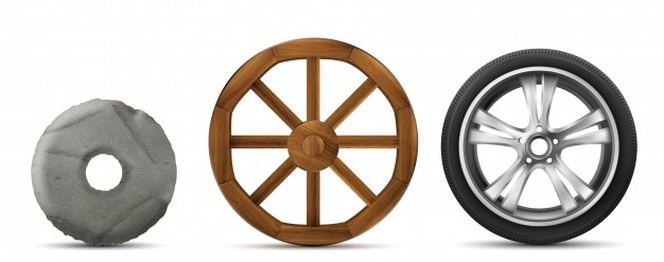
\includegraphics[width=0.79\textwidth]{img/plagiat/evolution-roue.jpg}
        \caption{
        L'évolution de la roue depuis son invention -3500 avant J.C (gauche), son allègement avec les inventions des roues à rayons en -2000 avant J.C (milieu), jusqu'aux roues à pneus en caoutchouc des véhicules que l'on utilise aujourd'hui (droite).
        }
        \label{fig:invention_roue}
    \end{figure}
\end{frame}
\begin{frame}{Simulation d'aquaplanage par Michelin}
    \begin{figure}
        \centering
        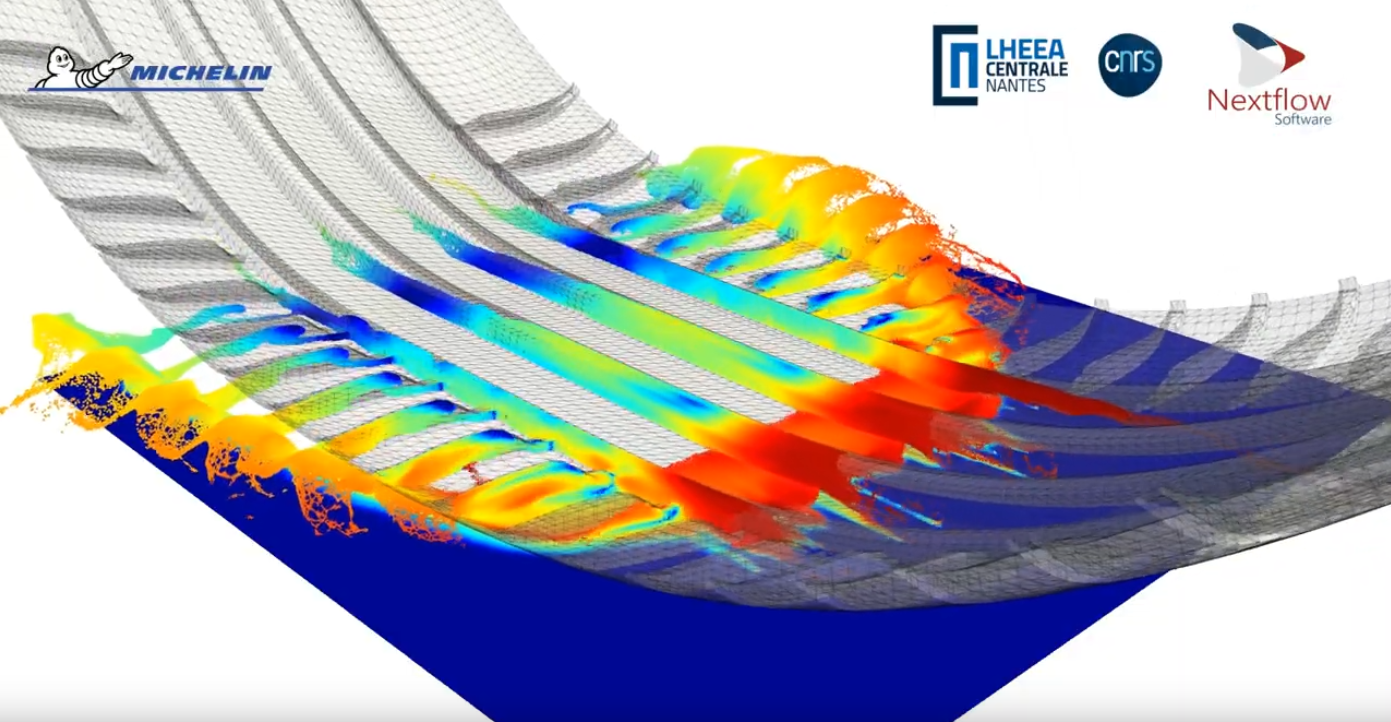
\includegraphics[width=0.79\textwidth]{img/plagiat/simulation_pneumatique_michelin.PNG}
        \caption{
            L'objectif est de s'assurer que les pneus développés par l'entreprise respectent les normes de sécurité en termes d'aquaplanage, 
            même lorsqu'ils sont usés. Image issue de \url{https://www.youtube.com/watch?v=S6csZMRy_xk}
        }
        \label{fig:simu_michelin}
    \end{figure}
\end{frame}


\begin{frame}{Simulation Numérique: Choix de la méthode}

    \begin{itemize}
        \item \only<1-5>{\textbf{Le modèle physique} \textcolor{darkgreen}{\footnotesize(hyperélasticité, plasticité, rupture)}}\only<6->{\textbf{Le modèle physique:} \textcolor{darkred}{\footnotesize{Choix: hyperélasticité}}}
        \item \only<2-5>{\textbf{La méthode numérique} \textcolor{darkgreen}{\footnotesize(méthode des éléments finies, différences finies, volumes finis)}}\only<6->{\textbf{La méthode numérique:} \textcolor{darkred}{\footnotesize{Choix: méthode des éléments finis}}}
        \item \only<3-5>{\textbf{La discrétisation en maillage} \textcolor{darkgreen}{\footnotesize(maillage triangulaire, quadrilatère, tétraèdrique, hexaédrique, hybride)}}\only<6->{\textbf{La discrétisation en maillage:} \textcolor{darkred}{\footnotesize{Choix: maillage quadrilatère / hexaédrique}}}
        \item \only<4-5>{\textbf{Les critères de convergence} \textcolor{darkgreen}{\footnotesize(critère de déplacement, critère de minimisation)}}\only<6->{\textbf{Les critères de convergence:} \textcolor{darkred}{\footnotesize{Choix: critère de déplacement et d'énergie sur une méthode de Newton}}}
        \item \only<5-5>{\textbf{Validation et vérification} \textcolor{darkgreen}{\footnotesize(comparaison des résultats avec des données de référence)}}\only<6->{\textbf{Validation et vérification:} \textcolor{darkred}{\footnotesize{Choix: si une simulation atteint l'itération finale, on la considère réussie}}}
    \end{itemize}

\end{frame}

\subsection{Critère de qualité d'un maillage hexaédrique pour ces simulations}

\begin{frame}
    \frametitle{Table des matières}
    \tableofcontents[currentsubsection, sectionstyle=show/shaded, subsectionstyle=show/shaded/hide]
\end{frame}
\begin{frame}{Définition et propriétés fondamentales du maillage}
    \small{
        \textbf{Définition :} Un maillage $\mathcal{M}$ décompose un domaine géométrique fermé $\Omega$ en un ensemble fini d'éléments simples $(\sigma_i)_N$. 
        \begin{align*}
            \Omega = \bigcup_{0 \leq i \leq N}{\sigma_i}
        \end{align*}
    }
    \newline
    \small{
        \textbf{Conformité :} Un maillage est conforme si l'intersection entre deux éléments adjacents est vide, un sommet commun, une arête commune ou une face commune.\\
    }
    \vspace{0.5cm}
    \small{
        \textbf{Description CAO :} Représentation numérique d'un objet dans un espace 2D ou 3D utilisant des entités géométriques primitives.
    }
\end{frame}
\begin{frame}{Un maillage conforme unique pour toute la simulation}
    \begin{columns}
    \column{0.5\textwidth}
    \small{
        \textbf{Objectif :} Un maillage unique pour toute la simulation, conservant une bonne qualité malgré les déformations.\\
    }
    \vspace{0.3cm}
    \small{
        \textbf{Avantage :} Les hexaèdres peuvent être déformés sans affecter leurs angles dièdres, contrairement aux tétraèdres.\\
    }
    \vspace{0.3cm}
    \small{
        \textbf{Défi :} Créer ces maillages complexes peut prendre plusieurs mois de travail ingénieur.\\
    }
    \column{0.5\textwidth}
        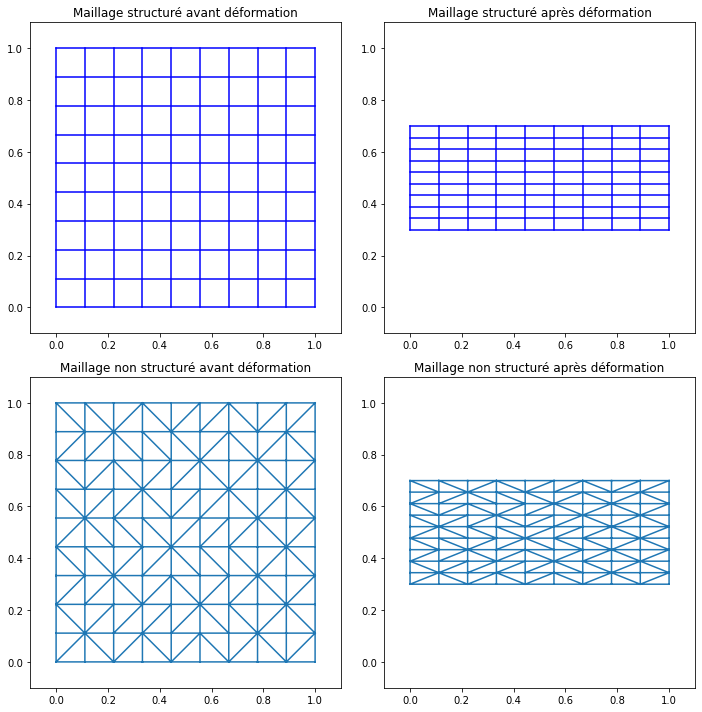
\includegraphics[width=\textwidth]{img/choix_maillage/deformation_low_angle.png}
    \end{columns}
    \end{frame}


\begin{frame}{Maillage hexaédrique de qualité pour ce type de simulation}
    \small{
        \textbf{Angles dièdres :} Entre 45 et 135 degrés pour éviter les problèmes de convergence.\\
    }
    \vspace{0.5cm}
    \small{
        \textbf{Rapport d'aspect :} Maximum de 100 entre la plus grande et la plus petite arête d'un hexaèdre.\\
    }
    \vspace{0.5cm}
    \small{
        \textbf{Alignement avec les bords :} Permet de préserver la qualité des angles pendant la simulation.\\
    }
    \vspace{0.5cm}
    \small{
        \textbf{Haute qualité localisée :} Crucial dans les zones à haut gradient de force pour minimiser les erreurs numériques.\\
    }
\end{frame}

\subsection{Maillage hexaédrique à partir d'un champ de repère}
\begin{frame}
    \frametitle{Table des matières}
    \tableofcontents[currentsubsection, sectionstyle=show/shaded, subsectionstyle=show/shaded/hide]
\end{frame}
\begin{frame}{Lien entre champ de repère 2D et maillage quadrilatère}
    \begin{center}
        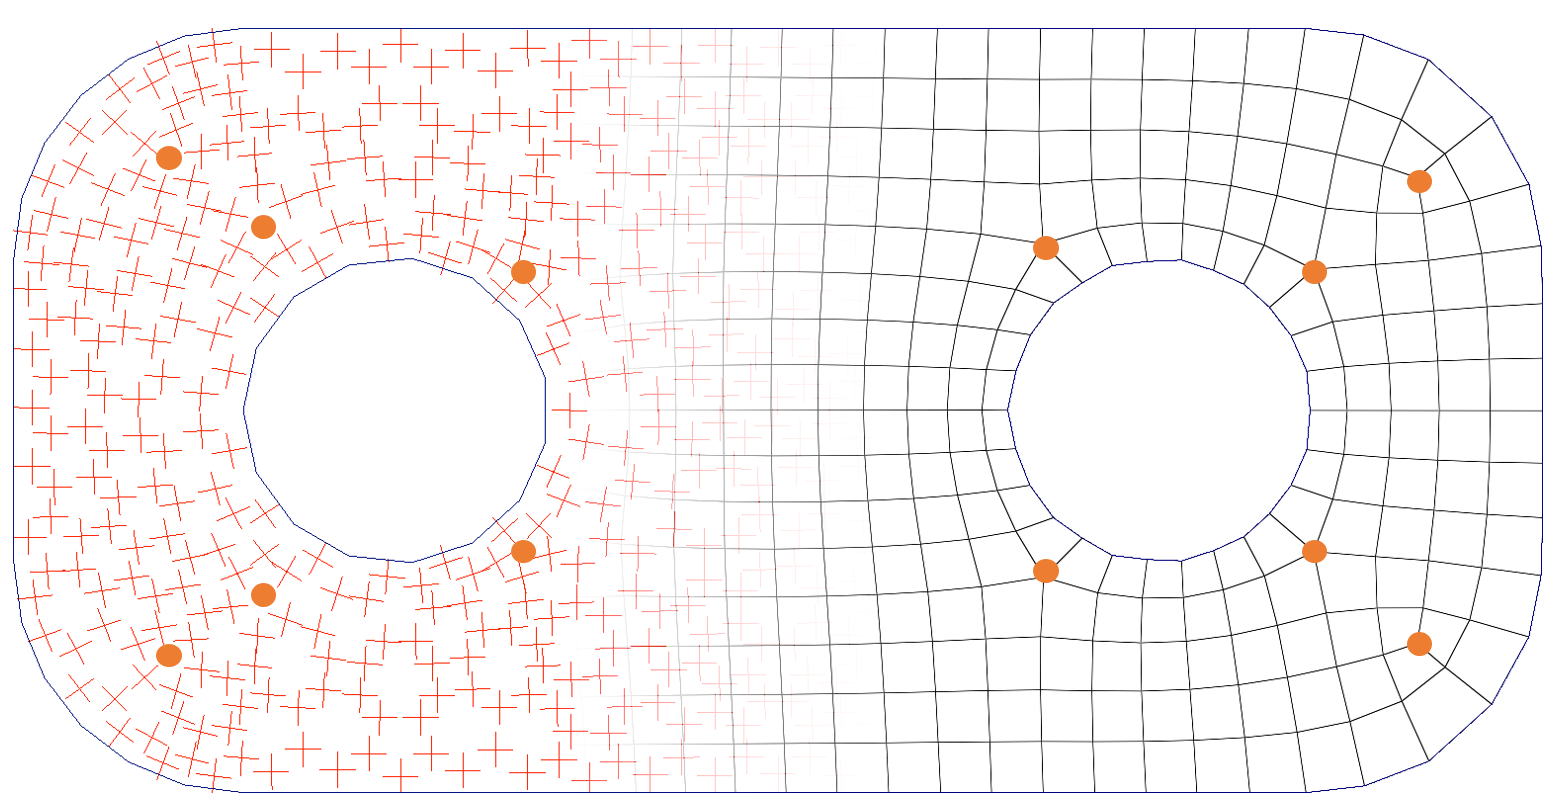
\includegraphics[width=\linewidth]{img/quadsimu/singus.PNG}
        \small{
            \textit{Les singularités d'un champ de repère sont utilisées pour déterminer la position des sommets de valence différente de 4 dans le maillage quadrilatère.}
        }
    \end{center}
\end{frame}
\begin{frame}{Quadcover pour générer un maillage quadrilatère}
    \begin{center}
        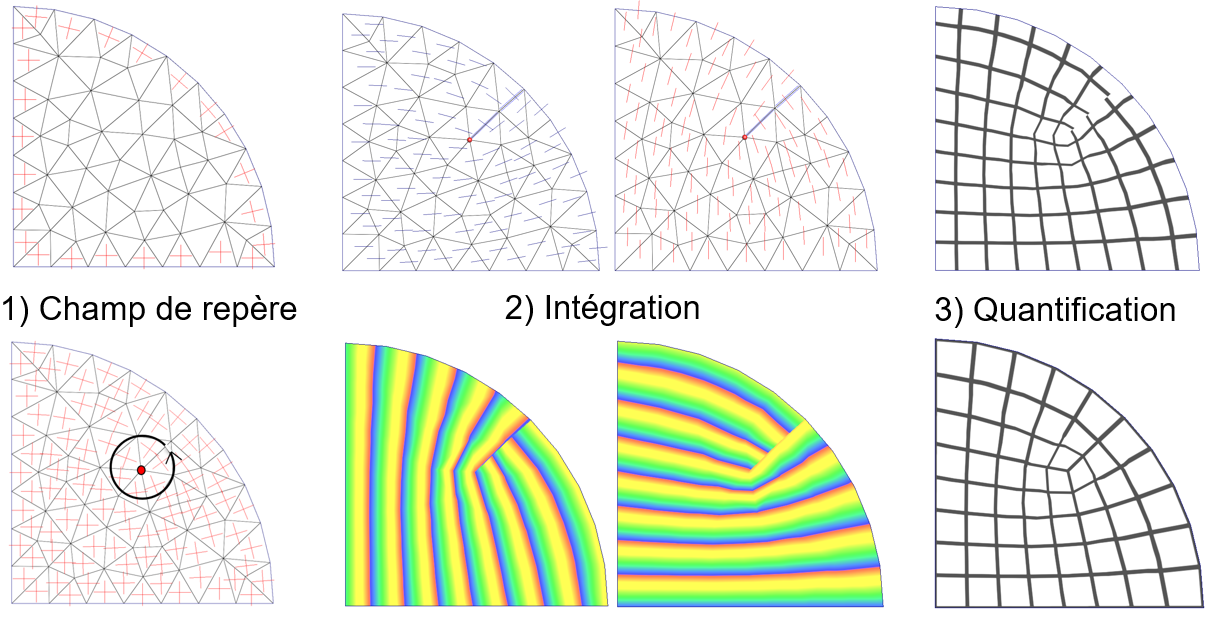
\includegraphics[width=\linewidth]{img/cubecover/pipeline.PNG}
        \small{
            \textit{Les différentes étapes de la méthode Quadcover pour construire un maillage quadrilatère.}
        }
    \end{center}
\end{frame}
\begin{frame}{En 3D: Cubecover pour générer un maillage hexaédrique}
    \begin{center}
        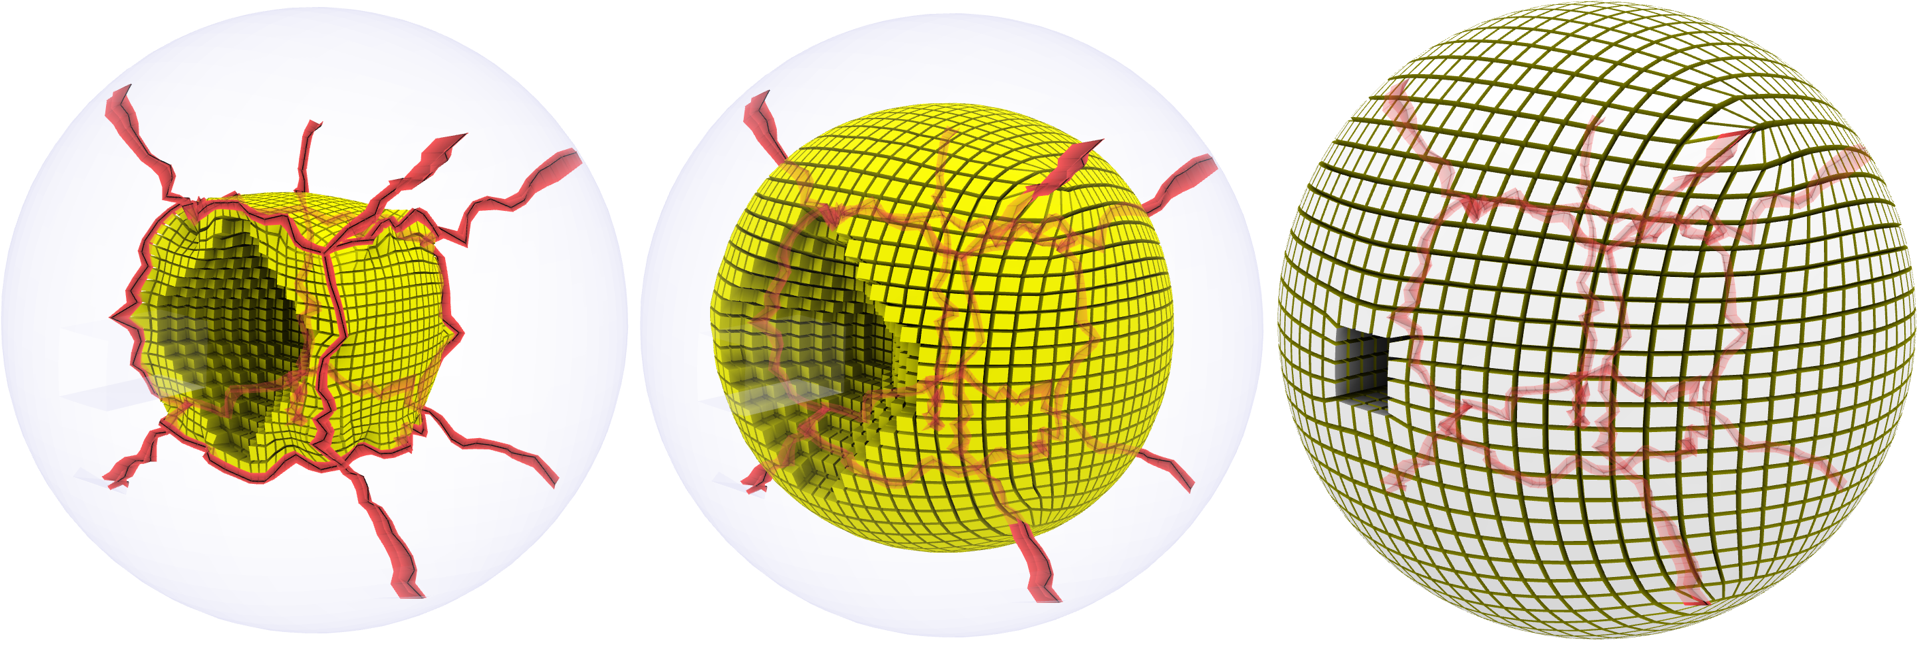
\includegraphics[width=\linewidth]{img/cubecover/B34_graphe_interieur.PNG}
        \small{
            \textit{Cubecover utilise le graphe de singularité d'un champ de repère 3D pour construire un maillage hexaédrique partageant le même graphe de singularité.}
        }
    \end{center}
\end{frame}
\section{Contribution: Champ de repère pour générer un maillage CAO }
\begin{frame}
    \frametitle{Table des matières}
    \tableofcontents[currentsection, sectionstyle=show/shaded, subsectionstyle=show/show/hide]
\end{frame}
\subsection{Champ 2D pour maillage quadrilatère de modèle CAO}
\begin{frame}
    \frametitle{Table des matières}
    \tableofcontents[currentsubsection, sectionstyle=show/shaded, subsectionstyle=show/shaded/hide]
\end{frame}

\begin{frame}{Repère orthogonal 2D}
    \small
    Un repère orthogonal 2D est une croix orientée par un angle $\theta$.
    \newline
    \newline
    \begin{minipage}{0.46\textwidth}
        \centering
        \begin{tikzpicture}[very thick, scale=.9]
            \draw[->, red] (.8, 0) arc (0:40:.8) node[right,pos=.66] {$\theta_1$};
            \draw[->] (180:1.2) -- (0:1.2);
            \draw[->] (-90:1.2) -- (90:1.2);
            \draw[->, green] (220:1.2) -- (40:1.2);
            \draw[->, green] (310:1.2) -- (130:1.2);
        \end{tikzpicture}
    \end{minipage}
    \hfill
    \begin{minipage}{0.46\textwidth}
        \centering
        \begin{tikzpicture}[very thick, scale=.9]
            \draw[->, red] (.8, 0) arc (0:130:.8) node[right,pos=.2] {$\theta_2$};
            \draw[->] (180:1.2) -- (0:1.2);
            \draw[->] (-90:1.2) -- (90:1.2);
            \draw[->, green] (220:1.2) -- (40:1.2);
            \draw[->, green] (310:1.2) -- (130:1.2);
        \end{tikzpicture}
    \end{minipage}
    
    \vfill
    
    \small
    Une croix étant $\pi/2$-périodique, nous la représentons par $(X, Y) = (\cos4\theta, \sin4\theta)$ pour éviter les problèmes de périodicité.
    \newline
    \newline
    \begin{minipage}{0.4\textwidth}
        \centering
        \begin{tikzpicture}[very thick, scale=.9]
            \draw[->, red] (.8, 0) arc (0:160:.8) node[right,pos=.3] {$4\theta_1$};
            \draw[->] (180:1.2) -- (0:1.2);
            \draw[->] (-90:1.2) -- (90:1.2);
            \draw[->, blue] (340:1.2) -- (160:1.2) node[right,pos=1.4] {$(X_1, Y_1)$};
        \end{tikzpicture}
    \end{minipage}
    \hfill
    \begin{minipage}{0.53\textwidth}
        \centering
        \begin{tikzpicture}[very thick, scale=.9]
            \draw[->, red] (.8, 0) arc (0:520:.8) node[right,pos=.1] {$4\theta_2$};
            \draw[->] (180:1.2) -- (0:1.2);
            \draw[->] (-90:1.2) -- (90:1.2);
            \draw[->, blue] (340:1.2) -- (160:1.2) node[right,pos=1.4] {$(X_2, Y_2)$};
        \end{tikzpicture}
    \end{minipage}
\end{frame}
\begin{frame}{Champ de repère 2D plat}
    \centering
    \begin{tikzpicture}[very thick, scale=.6]
    \node[text width=.4\linewidth] at (3, -1.4) {Nous contraignons les \color{red} repères de bords};
    \draw[blue, thick] (3, 0) -- (4, 2) -- (4, 4) -- (1.5, 4.5) -- (0, 5) -- (0, 3) -- (1.5, 4.5) -- (2, 3) -- (4, 4);
    \draw[blue, thick] (0, 3) -- (2, 3) -- (1.5, 1.5) -- (4, 2) -- (2, 3);
    \draw[green] (0, 3) -- (3, 0) -- (6, 3) -- (6, 6) -- (0, 6) -- cycle;
    \draw[red] (.55, 4.2) {}++ (0:.4) --+ (180:.8);
    \draw[red] (.55, 4.2) {}++ (90:.4) --+ (270:.8);
    \draw[red] (1.2, 2.5) {}++ (45:.4) --+ (225:.8);
    \draw[red] (1.2, 2.5) {}++ (135:.4) --+ (315:.8);
    \draw[red] (2.8, 1.1) {}++ (45:.4) --+ (225:.8);
    \draw[red] (2.8, 1.1) {}++ (135:.4) --+ (315:.8);
    \end{tikzpicture} \pause \qquad
    \begin{tikzpicture}[very thick, scale=.6]
    \node[text width=.4\linewidth] at (3, -1.4) {Puis minimisons la rotation entre repères voisins};
    \draw[blue, thick] (3, 0) -- (4, 2) -- (4, 4) -- (1.5, 4.5) -- (0, 5) -- (0, 3) -- (1.5, 4.5) -- (2, 3) -- (4, 4);
    \draw[blue, thick] (0, 3) -- (2, 3) -- (1.5, 1.5) -- (4, 2) -- (2, 3);
    \draw[green] (0, 3) -- (3, 0) -- (6, 3) -- (6, 6) -- (0, 6) -- cycle;
    \draw[red] (.55, 4.2) {}++ (0:.4) --+ (180:.8);
    \draw[red] (.55, 4.2) {}++ (90:.4) --+ (270:.8);
    \draw[red] (1.2, 2.5) {}++ (45:.4) --+ (225:.8);
    \draw[red] (1.2, 2.5) {}++ (135:.4) --+ (315:.8);
    \draw[red] (2.8, 1.1) {}++ (45:.4) --+ (225:.8);
    \draw[red] (2.8, 1.1) {}++ (135:.4) --+ (315:.8);
    \draw[] (2.4, 2.2) {}++ (55:.4) --+ (235:.8);
    \draw[] (2.4, 2.2) {}++ (145:.4) --+ (325:.8);
    \draw[] (3.4, 3.) {}++ (62:.4) --+ (242:.8);
    \draw[] (3.4, 3.) {}++ (152:.4) --+ (332:.8);
    \draw[] (1.2, 3.5) {}++ (68:.4) --+ (248:.8);
    \draw[] (1.2, 3.5) {}++ (158:.4) --+ (338:.8);
    \draw[] (2.3, 3.75) {}++ (65:.4) --+ (245:.8);
    \draw[] (2.3, 3.75) {}++ (155:.4) --+ (335:.8);
    \end{tikzpicture}
\end{frame}
\begin{frame}{Champ de repère 2D plat}
    \small
    Pour optimiser un champ de repère 2D plat sans problème de périodicité, nous optimisons 
    les vecteurs de représentations $(X, Y)$:
    \small{
    \begin{equation*}
    \begin{array}{ll}
    \underset{X, Y}{\argmin} & \underset{t \in T}{\displaystyle\sum} \underset{t' \in \mathcal{N}(t)}{\displaystyle\sum} \left|\left|\ \begin{pmatrix} X_{t'}\\ Y_{t'}\end{pmatrix} - \begin{pmatrix} X_{t}\\ Y_{t}\end{pmatrix} \right|\right|^2, \\
    \text{sous contrainte: } & \forall t \in T_b, \begin{pmatrix} X_{t}\\ Y_{t}\end{pmatrix} = \begin{pmatrix} \cos4\eta_t\\ \sin4\eta_t\end{pmatrix}.
    \end{array}
    \end{equation*}
    }
    Puis nous retrouvons les angles $\theta$ du champ de repère:
    $$ \forall t \in T,\ \  \theta_t = \frac{1}{4}\tan^{-1}\frac{Y_t}{X_t}$$

\end{frame}

\begin{frame}{Comparaison de repères dans deux plans différents}
    \begin{center}
    \begin{tikzpicture}[scale=2, transform shape]
    \coordinate (A) at (0,0);
    \coordinate (B) at (2,0);
    \coordinate (C) at (1,1.7);
    \coordinate (D) at (3,0.85);
    
    % Calculate the center of each triangle
    \coordinate (Center1) at ($ 0.333*(A) + 0.333*(B) + 0.333*(C) $);
    \coordinate (Center2) at ($ 0.333*(C) + 0.333*(B) + 0.333*(D) $);
    \coordinate (Ref1) at ($(Center1) + 0.5*(C) - 0.5*(B)$);
    \coordinate (Ref2) at ($(Center2) + 0.5*(C) - 0.5*(B)$);
    \coordinate (Ref3) at ($(Center1) - 0.5*(C) + 0.5*(B)$);
    \coordinate (Ref4) at ($(Center2) - 0.5*(C) + 0.5*(B)$);
    \coordinate (Ref5) at ($(Center1) + 0.5*(A) - 0.5*(B)$);
    \coordinate (Ref6) at ($(Center1) - 0.5*(A) + 0.5*(B)$);
    
    % Draw the shadows first
    \draw[drop shadow={shadow xshift=1.ex,shadow yshift=-1.ex}] (A) -- (B) -- (C) -- cycle;
    \draw[drop shadow={shadow xshift=1.ex,shadow yshift=-1.ex}] (B) -- (D) -- (C) -- cycle;
    
    % Then draw the triangles
    \fill[blue, opacity=0.3, shading=ball, ball color=blue] (A) -- (B) -- (C) -- cycle;
    \fill[red, opacity=0.3, shading=ball, ball color=red] (B) -- (D) -- (C) -- cycle;
    
    % Draw the green crosses
    \begin{scope}[overlay]
        \node at (Center1) [rotate=30, green, scale=2] {$\times$};
        \node at (Center2) [rotate=10, green, scale=2] {$\times$};
    \end{scope}

    % Highlight the common edge
    \draw[ultra thick] (B) -- (C);
    

    % Calculate the start of the arcs (cross arm ends)
    \coordinate (StartArc1) at ($(Center1) + (30+45:0.25)$);
    \coordinate (StartArc2) at ($(Center2) + (10+45:0.25)$);
    \coordinate (Arriv1) at ($(Center1) + 0.125*(C) - 0.125*(B)$);
    \coordinate (Arriv2) at ($(Center2) + 0.125*(C) - 0.125*(B)$);

    % Add the angles
    \only<2-2>{
        \draw[->] (StartArc1) to[bend right=30] (Arriv1);    
        \node[scale=0.8] at ($(Center1)!0.5!(StartArc1) + (0.,0.35)$) {$\theta_1$};
    }
    \only<2-3>{
        % Add the dotted lines
        \draw[dotted] (Ref3) -- (Ref1);
        \draw[dotted] (Ref4) -- (Ref2);

        \draw[->] (StartArc2) to[bend right=30] (Arriv2);
        \node[scale=0.8] at ($(Center2)!0.5!(StartArc2) + (0.,0.35)$) {$\theta_2$};
    }
    
    \coordinate (StartArc3) at ($(Center1) + (30+45:0.25)$);
    \coordinate (Arriv3) at ($(Center1) - 0.14*(A) + 0.14*(B)$);
    \only<3-3>{
        % Add the dotted lines
        \draw[dotted] (Ref5) -- (Ref6);
        
        % Calculate the start of the arcs (cross arm ends)
        
        % Add the angles
        \draw[->] (StartArc3) to[bend left=30] (Arriv3);
        \node[scale=0.8] at ($(Center1)!0.5!(StartArc3) + (0.25,0.2)$) {$\theta_1$};

        % Add alpha angle
        \coordinate (alphaStart) at ($(Center1) + 0.3*(C) - 0.3*(B)$);
        \coordinate (alphaEnd) at ($(Center1) - 0.3*(A) + 0.3*(B)$);
        \draw[->,red] (alphaStart) to[bend left=40] (alphaEnd);
        \node[red,scale=0.8] at ($(Center1)!0.5!(StartArc3) + (0.,0.5)$) {$\alpha_1$};
    }

    \only<4-4>{
        \draw[dotted] (Ref4) -- (Ref2);
        \draw[dotted] (Ref5) -- (Ref6);
        \draw[->] (StartArc3) to[bend left=30] (Arriv3);
        \node[scale=0.8] at ($(Center1)!0.5!(StartArc3) + (0.25,0.2)$) {$\theta_{t}$};
        \draw[->] (StartArc2) to[bend right=30] (Arriv2);
        \node[scale=0.8] at ($(Center2)!0.5!(StartArc2) + (0.,0.35)$) {$\theta_{t'}$};
         % Add omega
        \node[red, scale=0.8] at ($(B)!0.3!(C)$) {$\omega_{tt'}$};
    }
    
    \end{tikzpicture}
    \newline
    \only<1-1>{
        \newline
        Nous utilisons l'arête commune pour comparer les angles des repères par rapport à une même référence.
        %Problème: comment comparer des repères se situant dans deux plans différents ?\\ 
        %Nous allons utiliser l'arête partagée par les deux triangles comme référence d'angle.
    }
    \only<2-2>{
        Rotation entre les deux repères: $\theta_2 - \theta_1 \pmod{\pi/2}$
    }
    \only<3-3>{
        Rotation entre les deux repères: $\theta_2 - \theta_1 + \alpha_1 \pmod{\pi/2}$\\
        Ou plus généralement: $\theta_2 - \theta_1 - \alpha_2 + \alpha_1 \pmod{\pi/2}$
    }
    \only<4-4>{
        \newline
        Pour chaque paire de triangles adjacents $t, t'$, on définit:
        $$\omega_{tt'} = - \omega_{t't} = \alpha_{t'} - \alpha_{t}$$
        La rotation entre les repères de $t$ et $t'$ devient: 
        $$
            \theta_{t'} - \theta_{t} - \omega_{tt'} \pmod{\pi/2}
        $$
    }
    \end{center}


\end{frame}

\begin{frame}{Champ de repère 2D surfacique}
    \small
    Dans le cas surfacique, nous voulons minimiser les rotations:
    $$
        \theta_{t'} - \theta_{t} - \omega_{tt'} \pmod{\pi/2}
    $$

    Le problème d'optimisation devient alors :
    \small{
    \begin{equation*}
    \begin{array}{ll}
    \underset{X, Y}{\argmin} & \underset{t \in T}{\displaystyle\sum} \underset{t' \in \mathcal{N}(t)}{\displaystyle\sum} \left|\left|\ \begin{pmatrix} X_{t'}\\ Y_{t'}\end{pmatrix} - \begin{pmatrix}\cos4\omega_{tt'} & -\sin4\omega_{tt'} \\ \sin4\omega_{tt'} & \cos4\omega_{tt'} \end{pmatrix} \begin{pmatrix} X_{t}\\ Y_{t}\end{pmatrix} \right|\right|^2, \\
    \text{sous contrainte: } & \forall t \in T_b, \begin{pmatrix} X_{t}\\ Y_{t}\end{pmatrix} = \begin{pmatrix} \cos4\eta_t\\ \sin4\eta_t\end{pmatrix}.
    \end{array}
    \end{equation*}
    }
\end{frame}

\begin{frame}
    \frametitle{Maillages quadrilatères surfaciques}
    \begin{figure}
    \centering
    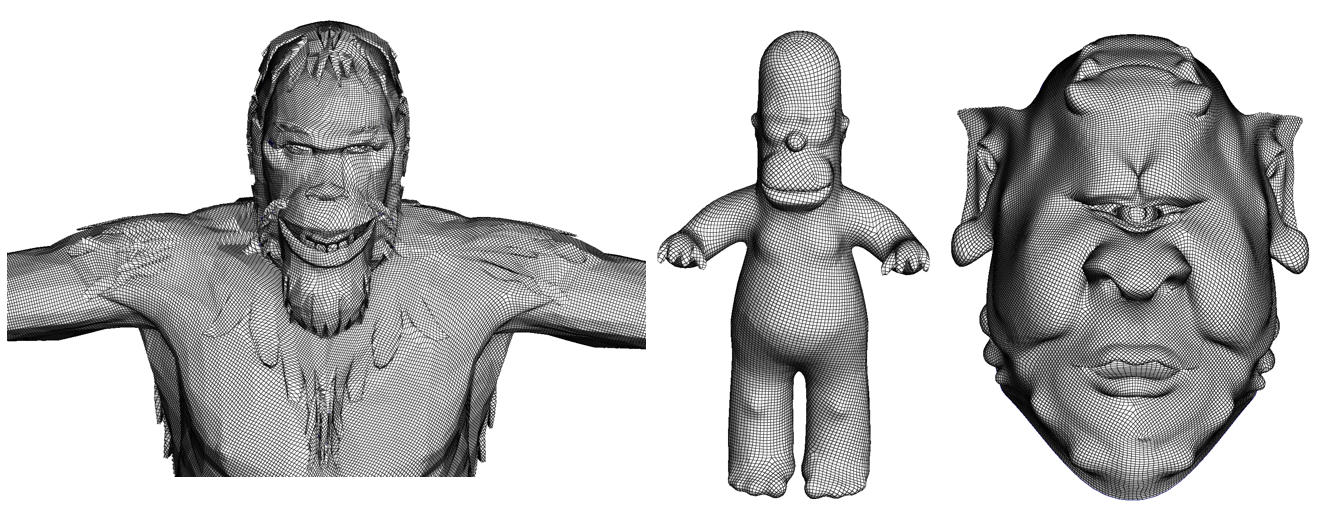
\includegraphics[width=\textwidth]{img/new_images/CG_models.PNG}
    \caption{Exemple de maillages quadrilatères surfaciques}
    \end{figure}
\end{frame}
    

\subsection{Champ 3D pour maillage hexaédrique de modèle CAO}
\begin{frame}
    \frametitle{Table des matières}
    \tableofcontents[currentsubsection, sectionstyle=show/shaded, subsectionstyle=show/shaded/hide]
\end{frame}
\subsection{Champ de repère non-orthogonal}
\begin{frame}
    \frametitle{Table des matières}
    \tableofcontents[currentsubsection, sectionstyle=show/shaded, subsectionstyle=show/shaded/hide]
\end{frame}

\begin{frame}{Repère 2D en tant que fonction polynomiale}
    \centering
    \vspace*{0.2\baselineskip}
    \small{
    $\mathcal{U} = \left\{\vec{u},\ -\vec{u},\ \vec{v},\ -\vec{v}\right\}$ est représenté par un polynôme \\
    \textbf{restreint à un cercle} \\
    \vspace*{0.45\baselineskip}
    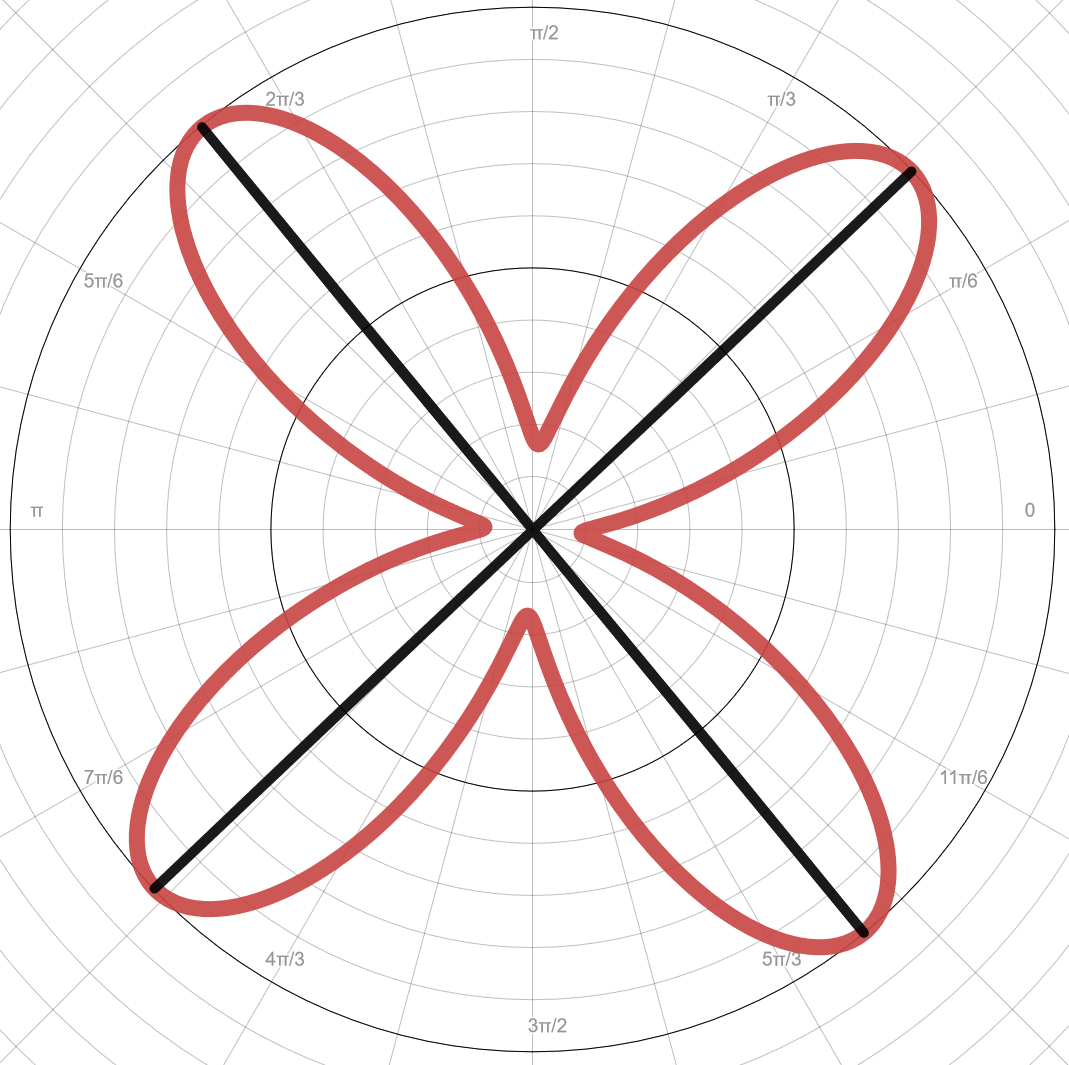
\includegraphics[width=0.36\linewidth]{img_spm_ff/poly_2D_8_2.PNG}
    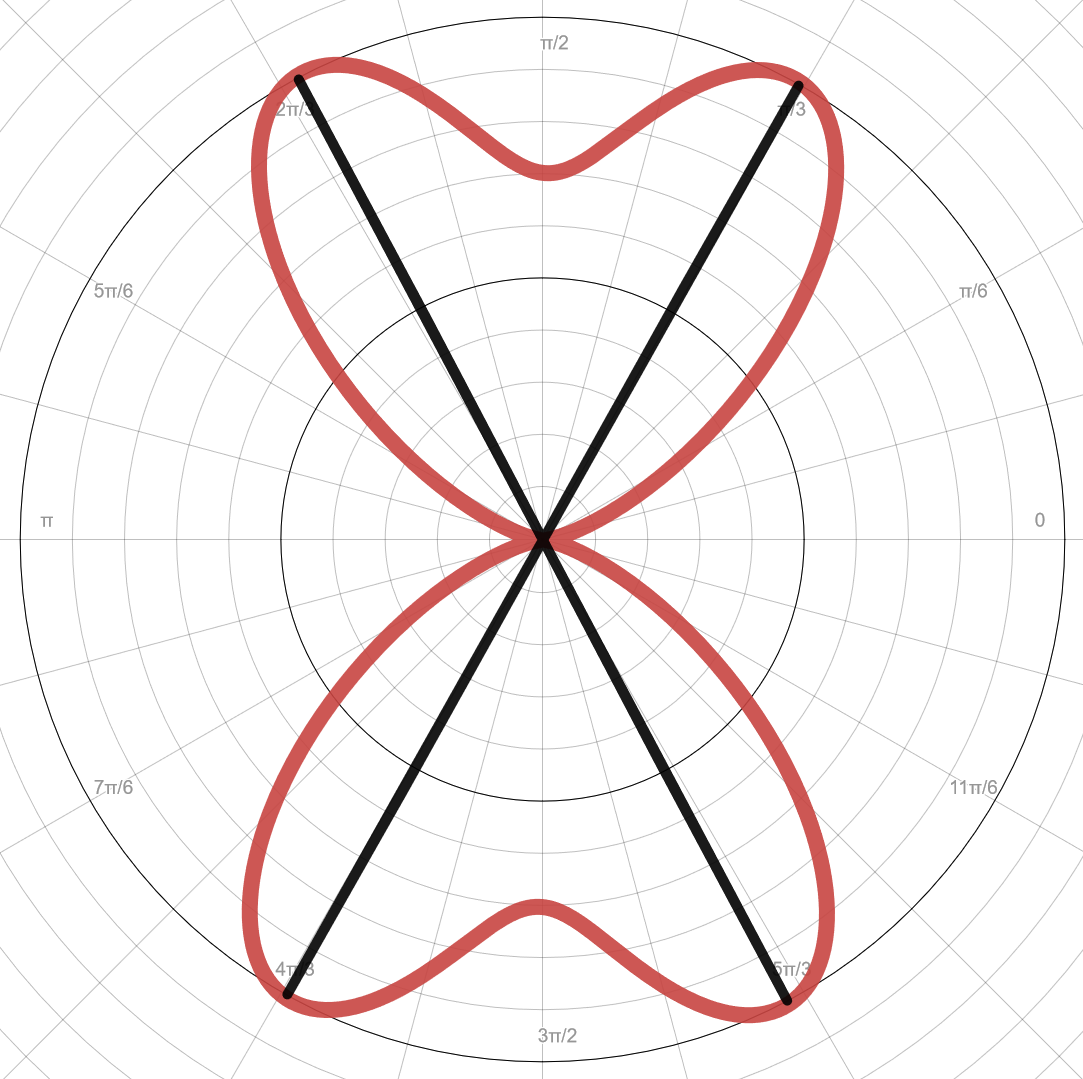
\includegraphics[width=0.36\linewidth]{img_spm_ff/poly_2D_8_1.PNG}
    
    \begin{itemize}
    \item Un polynôme restreint à un cercle donne les symétries désirées
    \item $dist(\mathcal{U}_i, \mathcal{U}_j) = \int (P_{\mathcal{U}_i} - P_{\mathcal{U}_j})^2$
    \item $P_\mathcal{U}$ a géométriquement la forme de $\mathcal{U}$ 
    \end{itemize}
    }
\end{frame}
\begin{frame}{Polynôme représentant un repère à 2 directions}
    \centering
    \small{
    $\mathcal{U} = \left\{\vec{u},\ -\vec{u},\ \vec{v},\ -\vec{v}\right\}$ est représenté par un polynôme \\
    \textbf{restreint à un cercle}
    }
    $$ P_\mathcal{U}(\vec{s}) = \langle \vec{u},\ \vec{s}\rangle^{4} +  \langle \vec{v},\ \vec{s}\rangle^{4}, \ \ \   \forall \vec{s} \in {\rm I\!R}^2, \lVert \vec{s} \rVert = 1$$
    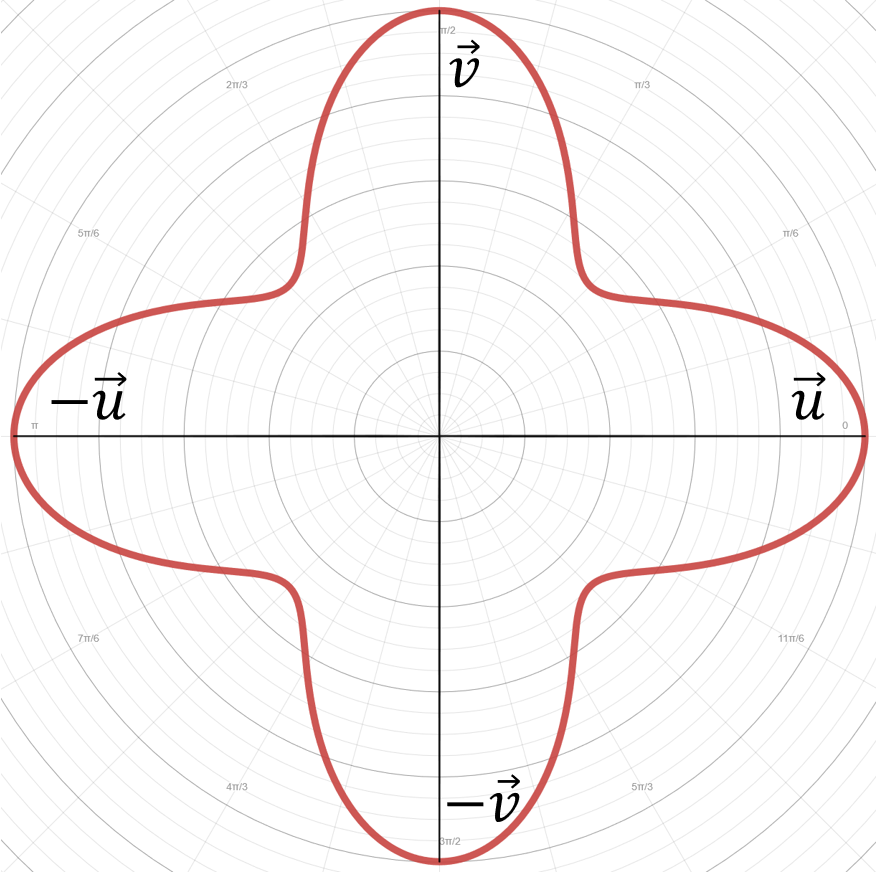
\includegraphics[width=0.4\linewidth]{img_spm_ff/anoted_orthogonal.PNG}
    \ \ \ 
    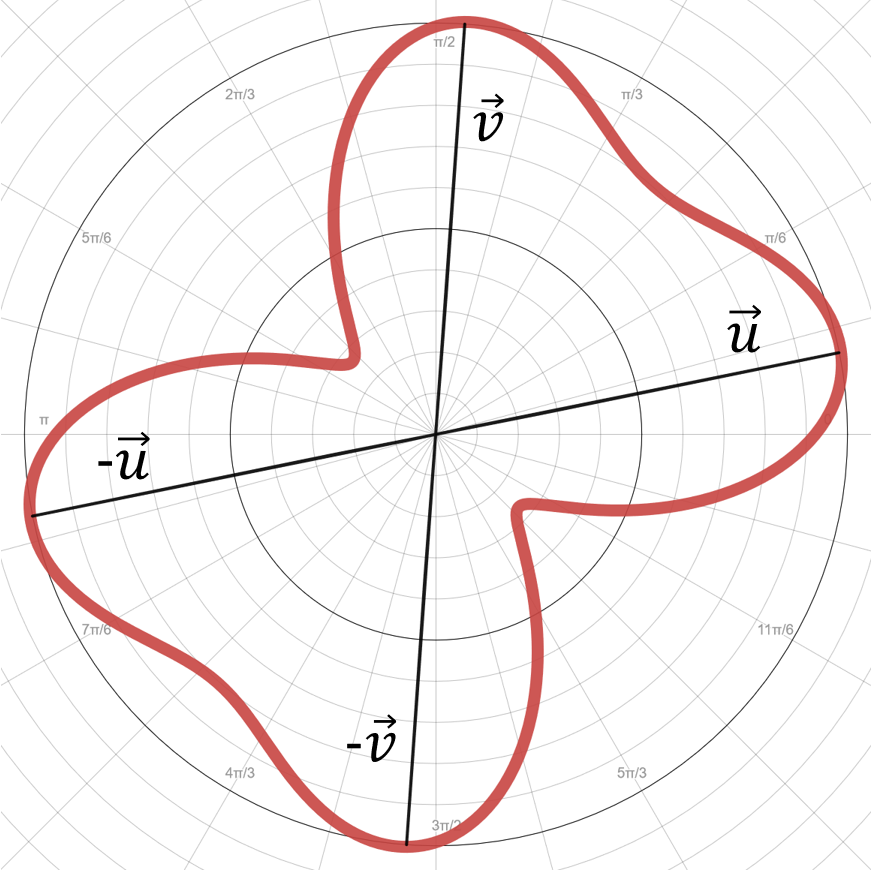
\includegraphics[width=0.4\linewidth]{img_spm_ff/anoted_polynome.PNG}
\end{frame} 
\begin{frame}{Décomposition dans la base de Fourier}
    \centering
    \begin{overprint}
    \onslide<1> \centering
    Les polynômes de repères 2D orthogonaux peuvent être décomposés dans la base de Fourier comme suit :
    
    \vspace*{0.5\baselineskip}
    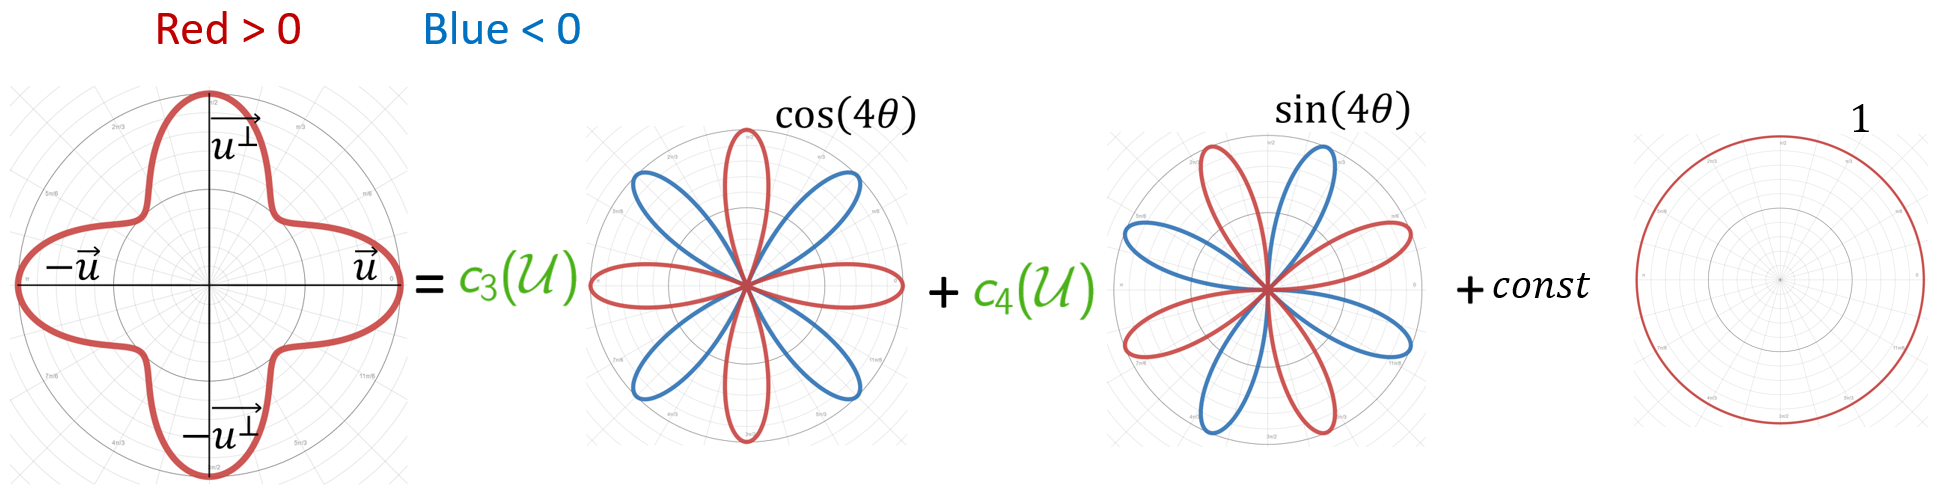
\includegraphics[width=0.95\linewidth]{img_spm_ff/ortho_decomposition_with_circle.PNG}
    
    $$ dist(\mathcal{U}_i, \mathcal{U}_j) =  \int (P_{\mathcal{U}_i} - P_{\mathcal{U}_j})^2 =  \left({\color{green}c_3(\mathcal{U}_i)} - {\color{green}c_3(\mathcal{U}_j)} \right)^2 
    + \left({\color{green}c_4(\mathcal{U}_i)} - {\color{green}c_4(\mathcal{U}_j)} \right)^2$$
    \onslide<2> \centering
    Les termes du $2^{nd}$ ordre sont nécessaires pour la non-orthogonalité
    
    \vspace*{0.5\baselineskip}
    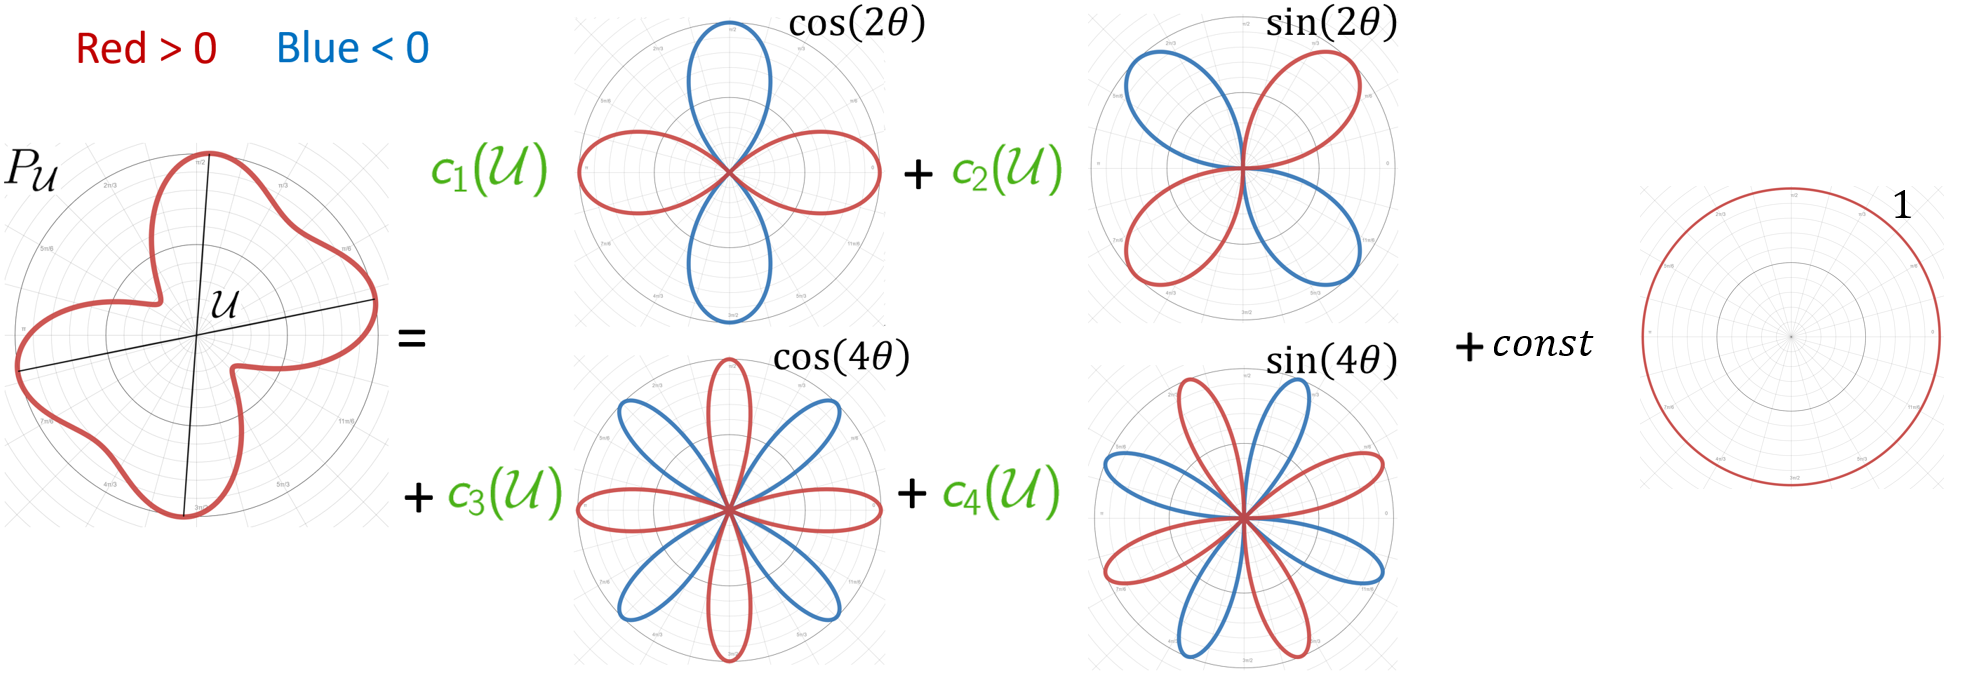
\includegraphics[width=0.95\linewidth]{img_spm_ff/polynome_decomposition_with_circle.PNG}
    $$ dist(\mathcal{U}_i, \mathcal{U}_j) =  \int (P_{\mathcal{U}_i} - P_{\mathcal{U}_j})^2 = \sum_{\ell=1}^4 \left({\color{green}c_\ell(\mathcal{U}_i)} - {\color{green}c_\ell(\mathcal{U}_j)} \right)^2$$
    \end{overprint}
\end{frame} 
\begin{frame}{2D Optimization}
    \centering
    \small
    %From the decomposition in the Fourier basis, we define
    %$$ dist(\mathcal{U}_i, \mathcal{U}_j) =  \int (P_{\mathcal{U}_i} - P_{\mathcal{U}_j})^2 = \sum_{\ell=1}^4 \left({\color{green}c_\ell(\mathcal{U}_i)} - {\color{green}c_\ell(\mathcal{U}_j)} \right)^2$$
    Pour calculer un champ de repère non-orthogonal 2D lisse, nous minimisons avec LBFGS l'énergie suivante :
    $$ E_{tot} = \sum_{Voisins(i, j)} dist(\mathcal{U}_i, \mathcal{U}_j)$$
    
    Contrôle de l'orthogonalité: $c_1, c_2, c_3, c_4 \mapsto \lambda c_1, \lambda c_2, c_3, c_4$ 
     
     \vspace*{0.5\baselineskip}
     %modifies the orthogonality of the field : 
    \begin{minipage}[b]{0.15\textwidth}
        \centering
        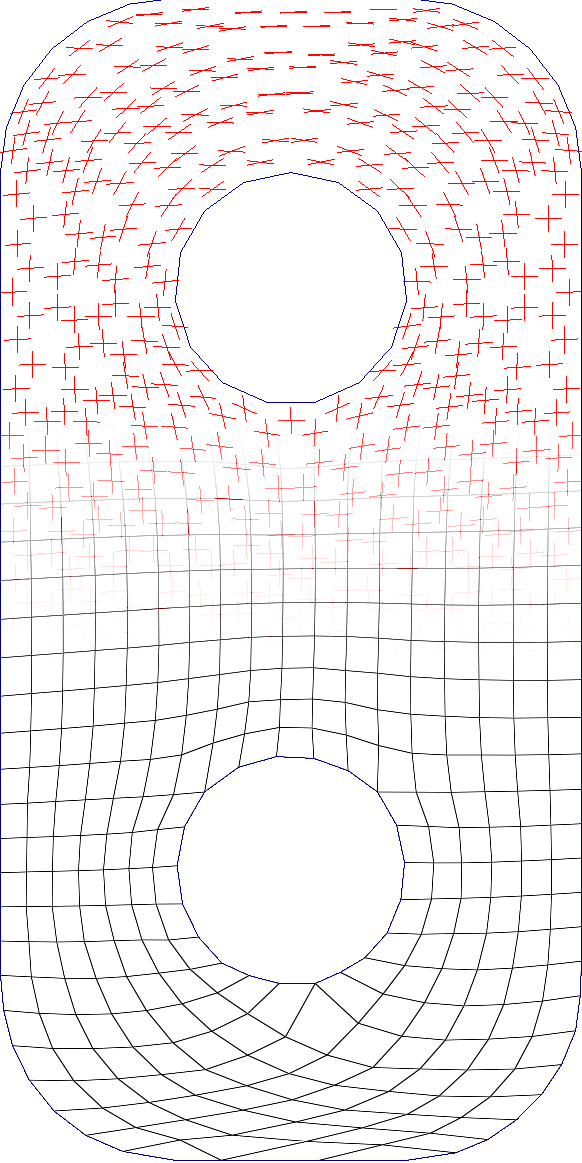
\includegraphics[width=\textwidth]{img_spm_ff/perced_1}
        $\lambda = 0.1$
    \end{minipage}
    \ \ \ 
    %\hfill
    \begin{minipage}[b]{0.15\textwidth}
        \centering
        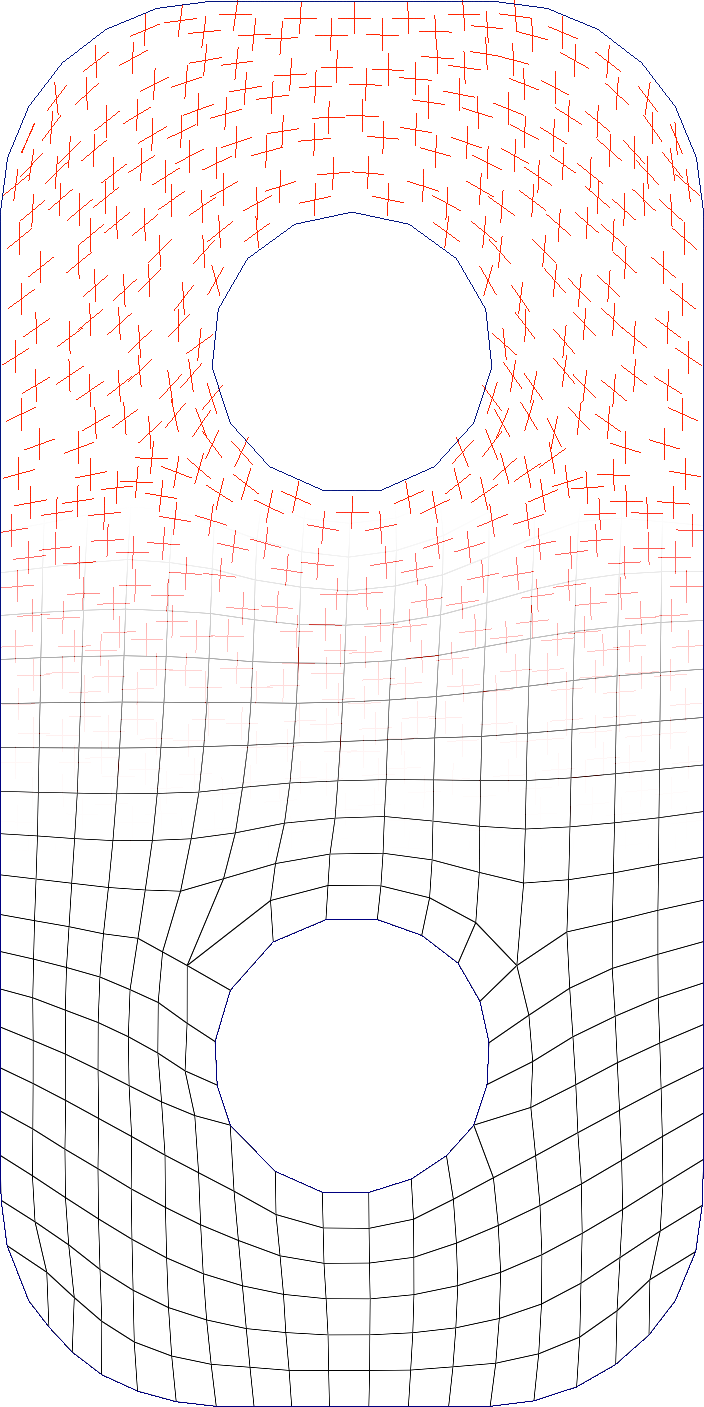
\includegraphics[width=\textwidth]{img_spm_ff/perced_9}
        $\lambda = 0.5$
    \end{minipage}
    %\hfill
    \ \ \ 
    \begin{minipage}[b]{0.15\textwidth}
        \centering
        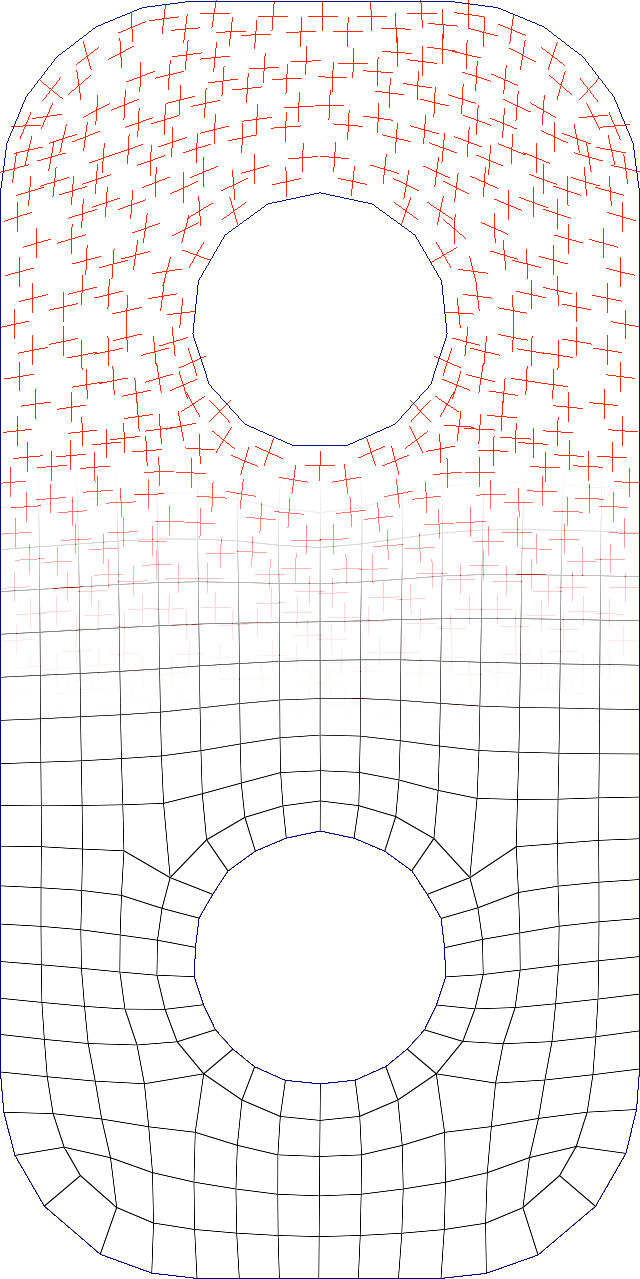
\includegraphics[width=\textwidth]{img_spm_ff/perced_16}
        $\lambda = 1$
    \end{minipage}
    %\hfill
    \ \ \ 
    \begin{minipage}[b]{0.15\textwidth}
        \centering
        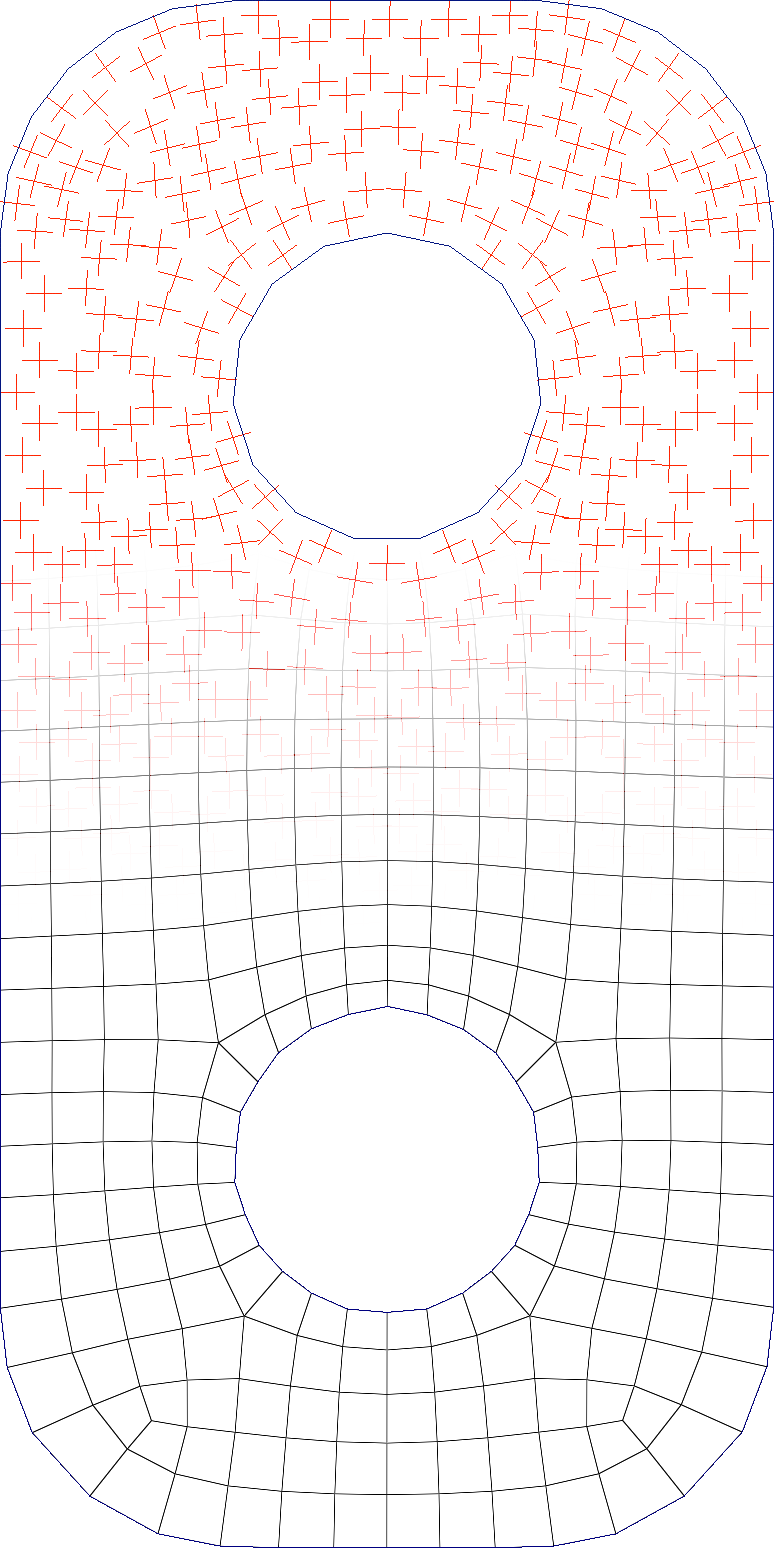
\includegraphics[width=\textwidth]{img_spm_ff/perced_25}
        $\lambda = 1.5$
    \end{minipage}
\end{frame} 

\begin{frame}{2D Results}
    \centering
    
    \begin{minipage}[c]{0.45\textwidth}
    \centering 
    \textbf{Orthogonal fields}
    \vspace*{1\baselineskip}
    
     \includegraphics[width=0.7\linewidth]{img_spm_ff/quads_ortho_shurik0.PNG}
    \includegraphics[width=0.8\linewidth]{img_spm_ff/q_2_ortho_fail.PNG}
    %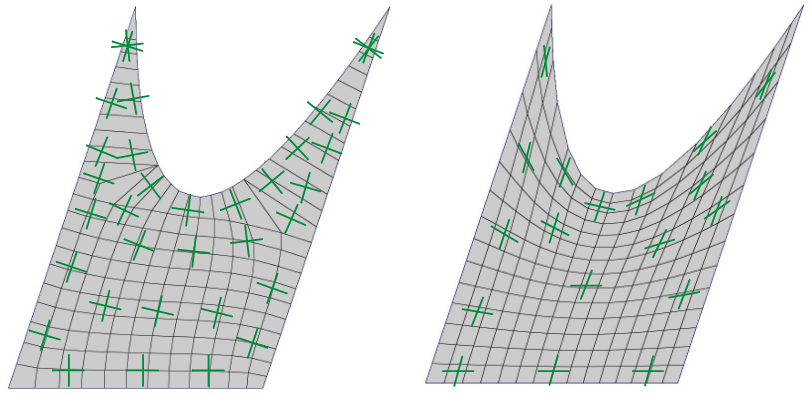
\includegraphics[width=.9\linewidth]{comp1.png}
    \end{minipage}%
    \hfill\vline\hfill
    \begin{minipage}[c]{0.45\textwidth}
    \centering 
    \textbf{Non-orthogonal fields}
    \vspace*{1\baselineskip}
    
    \includegraphics[width=0.7\linewidth]{img_spm_ff/quads_nonortho_shurik0.PNG}
    \includegraphics[width=0.8\linewidth]{img_spm_ff/q_2.PNG}
    \end{minipage}
\end{frame} 
\begin{frame}{Polynôme représentant un repère à 3 directions}
    \centering
    \small
    $\mathcal{U} = \left\{\vec{u},\ -\vec{u},\ \vec{v},\ -\vec{v},\ \vec{w},\ -\vec{w}\right\}$ est représenté par un polynôme \\
    \textbf{restreint à un cercle}
    %$$P_\mathcal{U} \colon s \mapsto \langle \vec{u},\ s\rangle^{4} +  \langle \vec{v},\ s\rangle^{4} +  \langle \vec{w},\ s\rangle^{4}$$
    $$ P_\mathcal{U}(\vec{s}) = \langle \vec{u},\ \vec{s}\rangle^{4} +  \langle \vec{v},\ \vec{s}\rangle^{4} +  \langle \vec{w},\ \vec{s}\rangle^{4}, \ \ \   \forall \vec{s} \in {\rm I\!R}^3, \lVert \vec{s} \rVert = 1$$
    
    \vspace*{.5\baselineskip}
    \includegraphics[width=0.33\linewidth]{img_spm_ff/sperical_3dir4.png}
    \ \ \ \ \ \ \ \ \ \ \ 
    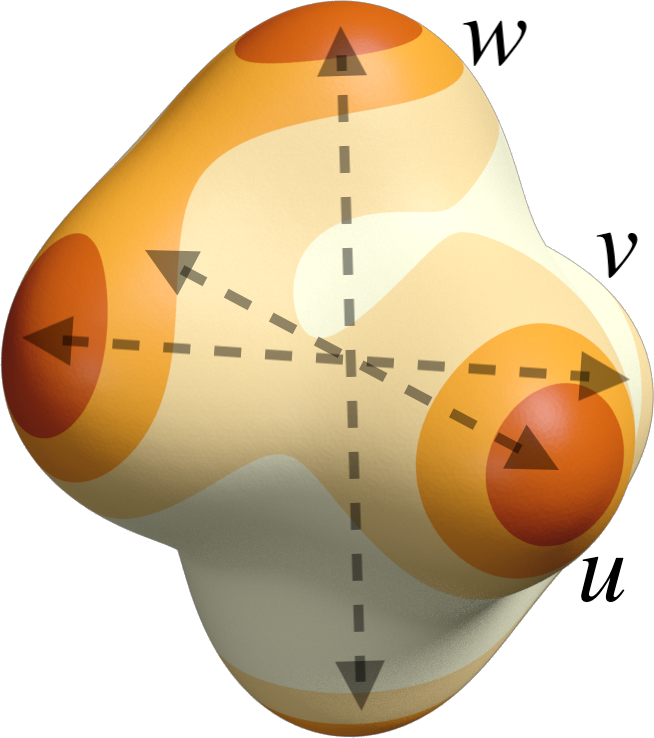
\includegraphics[width=0.3\linewidth]{img_spm_ff/sperical_3dir4_rot.png}
    %\begin{align*}
     %  p_c \colon & s \mapsto \langle u,\ s\rangle^{4} +  \langle v,\ s\rangle^{4} +  \langle w,\ s\rangle^{4} \\
     %  & \mathcal{S}_{\{0, 1\}}^3 \to {\rm I\!R}
    %\end{align*}
\end{frame} 
\begin{frame}{Décomposition dans la base des Harmoniques Sphériques}
    \centering
    \begin{overprint}
    \onslide<1> \centering
    \small
    Les polynômes de repères 3D orthogonaux peuvent être décomposés dans la base des Harmoniques Sphériques comme suit :\\
    \begin{minipage}[c]{0.24\textwidth}
        \centering
          \vspace*{.5\baselineskip}
          \hfill
        \includegraphics[width=0.6\linewidth]{img_spm_ff/sperical_3dir4.png}
    \end{minipage}
    \begin{minipage}[c]{0.74\textwidth}
        $$P_\mathcal{U}(s) = const \cdot Y_{0, 0} + \sum_{m = -4}^4{{\color{green}c_{4, m}(\mathcal{U})}Y_{4,m}(s)}$$ 
    \end{minipage}
    
    \vspace*{.5\baselineskip}
    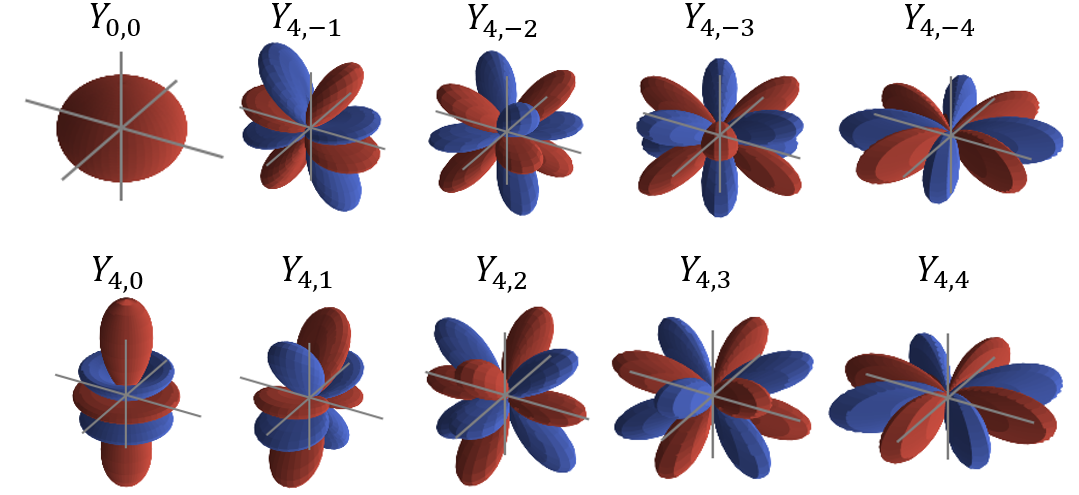
\includegraphics[width=.8\linewidth]{img_spm_ff/ortho_harmonic_decompo.PNG} 
    
    \onslide<2> \centering
    
    \small
    Les termes du $2^{nd}$ ordre sont nécessaires pour la non-orthogonalité:
    %$$P_\mathcal{U}(s) = const \cdot Y_{0, 0} + \sum_{\ell \in \{2, 4\}} \sum_{m = -\ell}^\ell{{\color{green}c_{\ell, m}(\mathcal{U})}Y_{\ell,m}(s)}$$ 
    
    \begin{minipage}[c]{0.19\textwidth}
        \centering
          \vspace*{.5\baselineskip}
          \hfill
        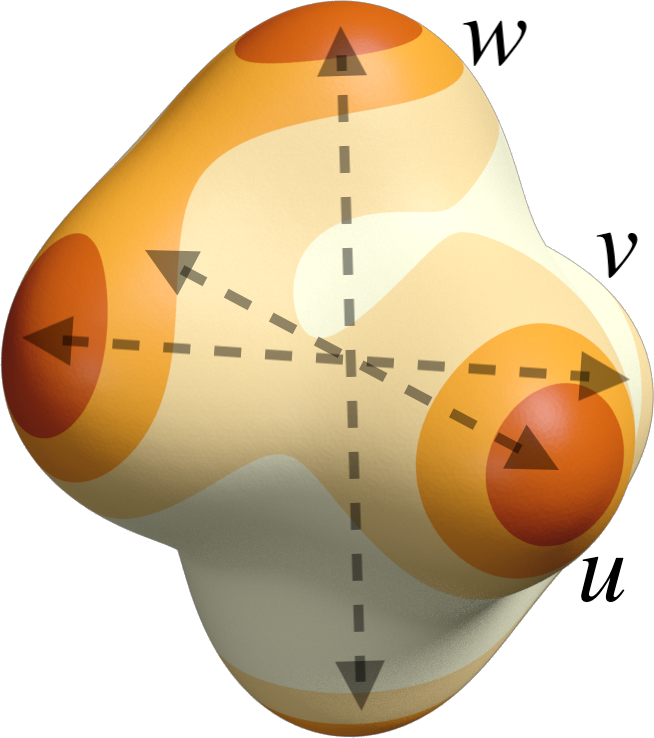
\includegraphics[width=0.8\linewidth]{img_spm_ff/sperical_3dir4_rot.png}
    \end{minipage}
    \begin{minipage}[c]{0.79\textwidth}
        %\centering
        %\includegraphics[width=0.33\linewidth]{sperical_3dir4.png}
        %$$P_\mathcal{U}(s) = const \cdot Y_{0, 0} + \sum_{m = -4}^4{{\color{green}c_{4, m}(\mathcal{U})}Y_{4,m}(s)}$$ 
        $$P_\mathcal{U}(s) = const \cdot Y_{0, 0} + \sum_{\ell \in \{2, 4\}} \sum_{m = -\ell}^\ell{{\color{green}c_{\ell, m}(\mathcal{U})}Y_{\ell,m}(s)}$$ 
    \end{minipage}
    
    \vspace*{.5\baselineskip}
    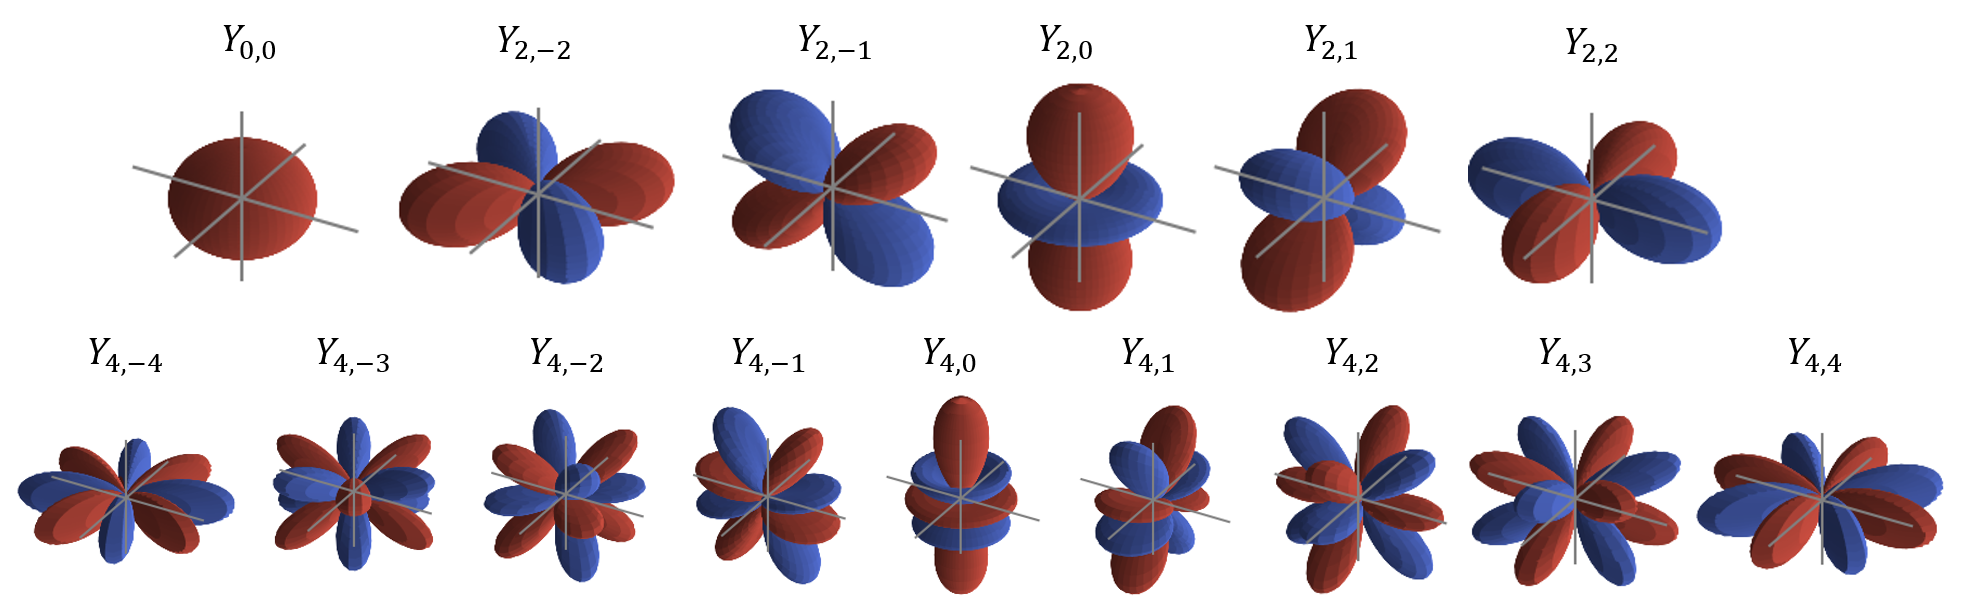
\includegraphics[width=\linewidth]{img_spm_ff/all_sph_harm.PNG} 
    \end{overprint}
\end{frame} 
\begin{frame}{Optimisation d'un champ de repère non-orthogonal 3D}
    \centering
    \footnotesize
     De la décomposition dans la base des Harmoniques, nous définissons:
    $$ dist(\mathcal{U}_i, \mathcal{U}_j) = \int (P_{\mathcal{U}_i} - P_{\mathcal{U}_j})^2 = \sum_{\ell, m} \left({\color{green}c_{\ell,m}(\mathcal{U}_i)} - {\color{green}c_{\ell,m}(\mathcal{U}_j)} \right)^2$$
    Pour calculer un champ de repère non-orthogonal 3D lisse, nous minimisons avec LBFGS l'énergie suivante :
    %To compute smoothed frame field, we minimize with LBFGS 
    $$ E_{tot} = \sum_{Voisins(i, j)} dist(\mathcal{U}_i, \mathcal{U}_j)$$
    %\vspace*{.5\baselineskip}
    %As in 2D, $\forall m,\ \ c_{2,m} \mapsto \lambda c_{2,m}$ modifies the orthogonality of the field. 
    Contrôle de l'orthogonalité: $\ \ c_{2,m} \mapsto \lambda c_{2,m} \ \ \ \ \ (-2 \leq m \leq 2)$ %modifies the orthogonality of the field. 
    
    \begin{minipage}[b]{0.33\textwidth}
        \centering
        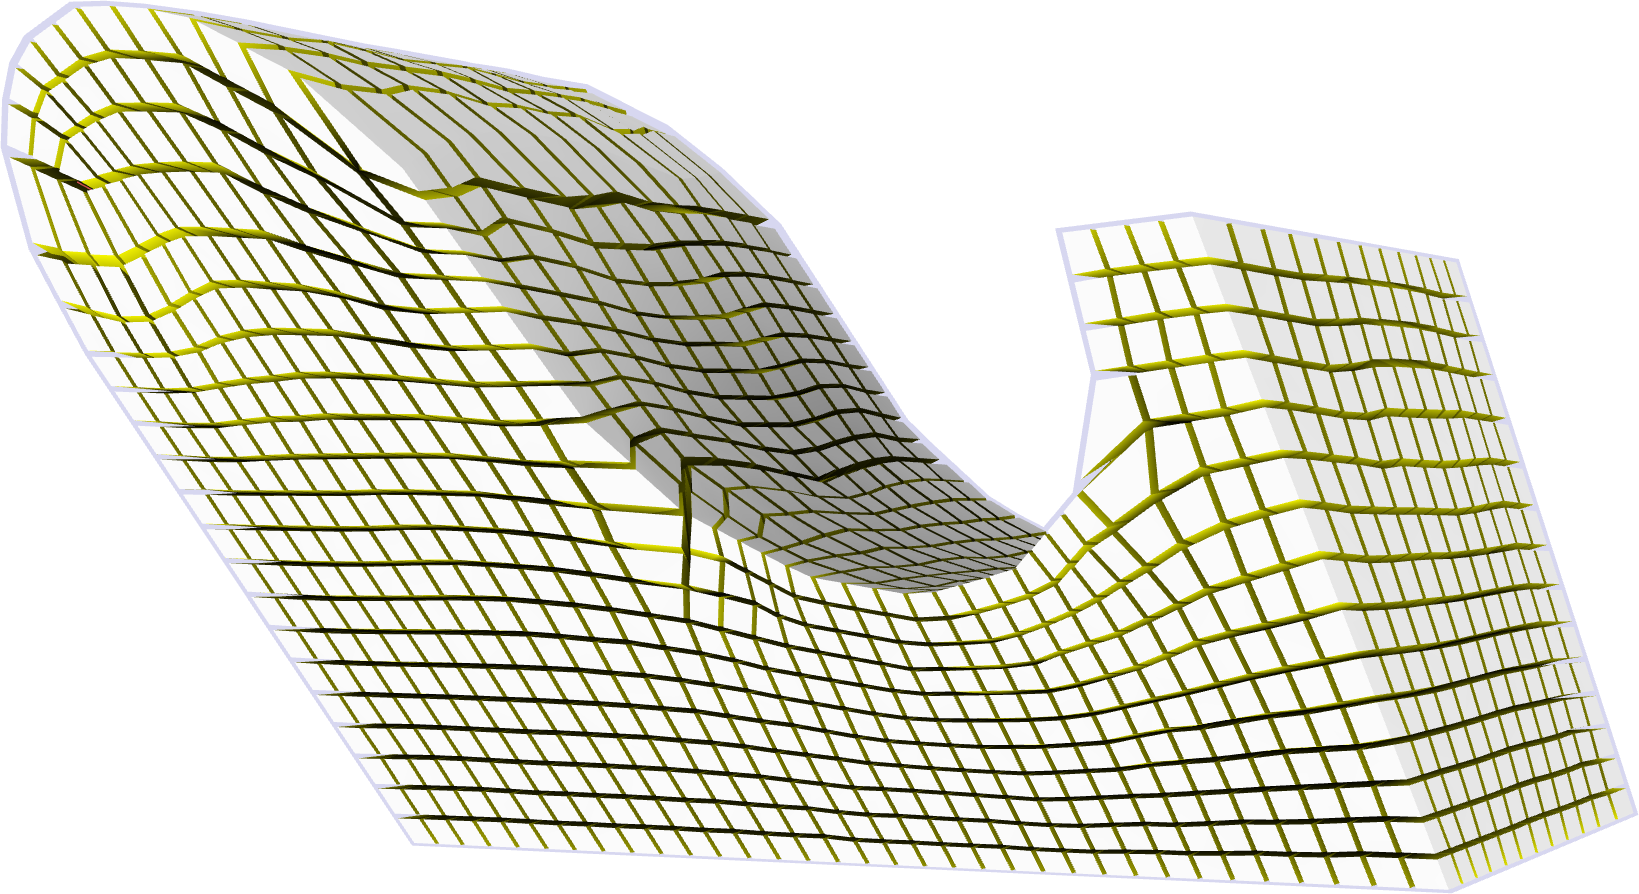
\includegraphics[width=\textwidth]{img_spm_ff/shear_0_7.png}
        $\lambda = 0.7$
    \end{minipage}
    \begin{minipage}[b]{0.28\textwidth}
        \centering
        \includegraphics[width=\textwidth]{img_spm_ff/shear_1.png}
        $\lambda = 1$
    \end{minipage}
    
    \normalsize
\end{frame} 
\begin{frame}{3D Results}
    \centering
    \begin{minipage}[c]{0.45\textwidth}
    \centering 
    \textbf{Champs orthogonaux}
    \vspace*{1\baselineskip}
    
     %\includegraphics[width=0.8\linewidth]{quads_ortho_shurik0.PNG}
    %\includegraphics[width=0.8\linewidth]{q_2_ortho_fail.PNG}
    
    \includegraphics[width=.66\linewidth]{img_spm_ff/shear_ortho.png}
    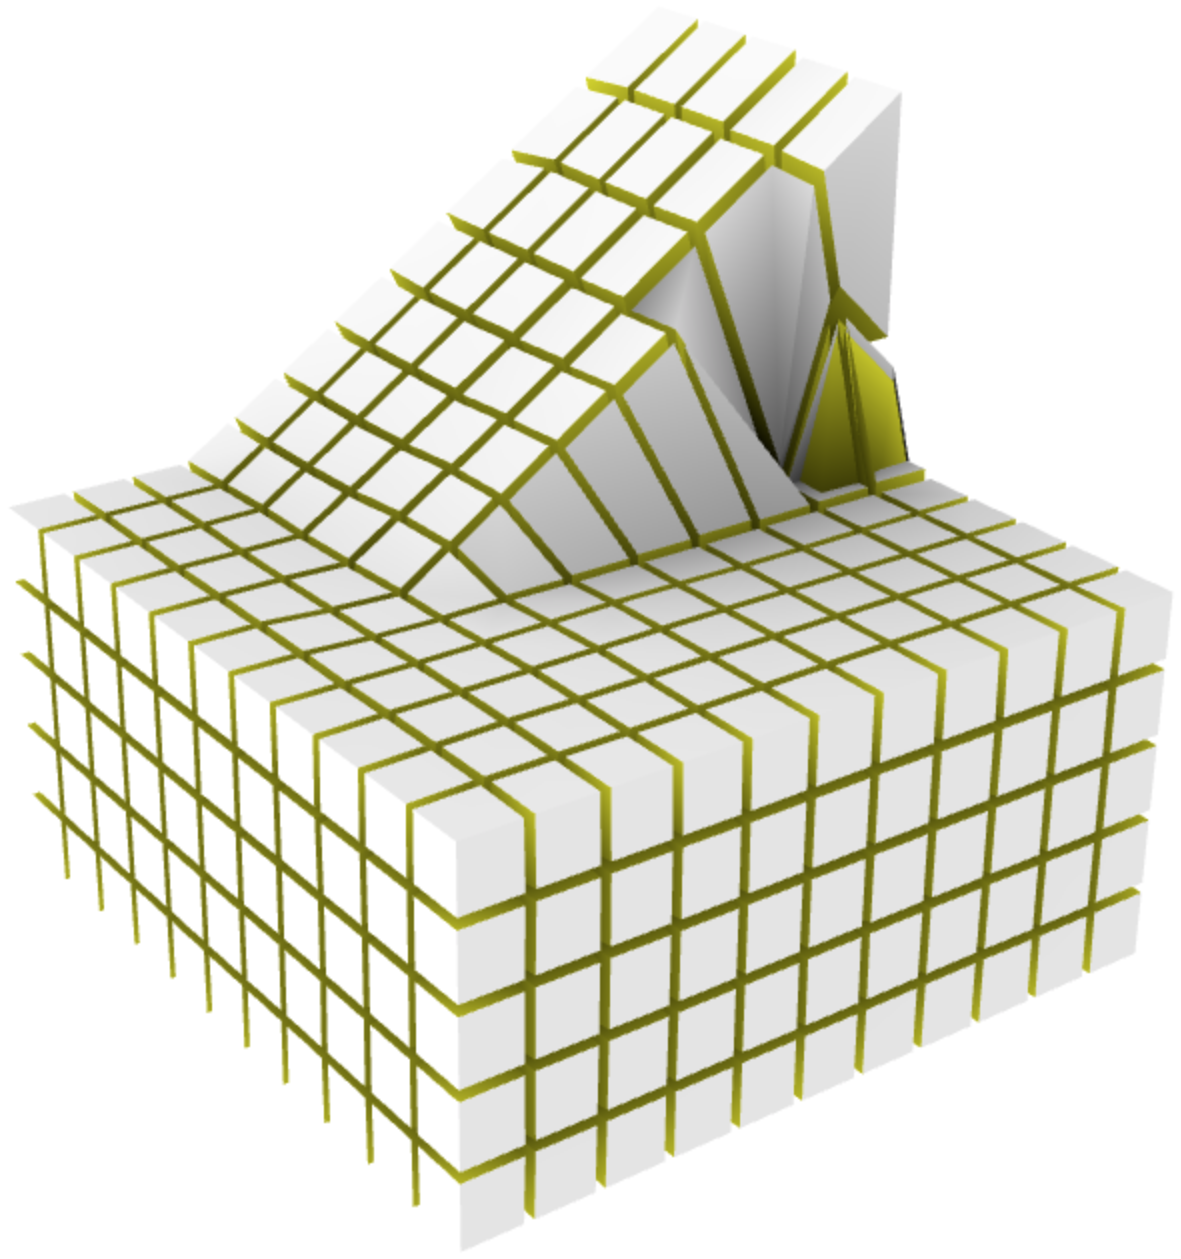
\includegraphics[width=.66\linewidth]{img_spm_ff/slope_ortho_front.png}
    %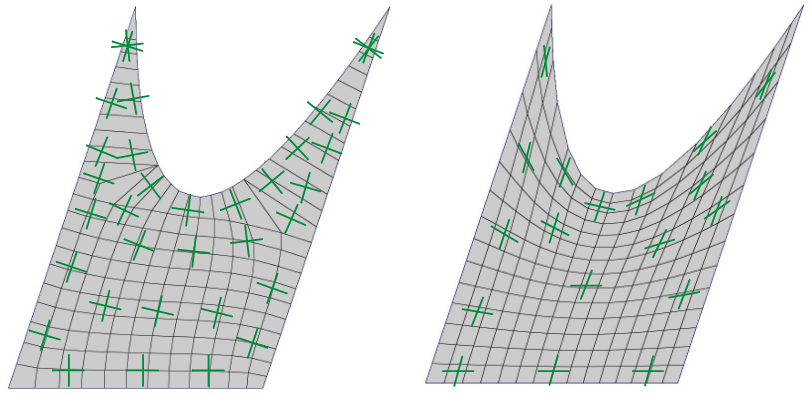
\includegraphics[width=.9\linewidth]{comp1.png}
    \end{minipage}%
    \hfill\vline\hfill
    \begin{minipage}[c]{0.45\textwidth}
    \centering 
    \textbf{Champs non-orthogonaux}
    \vspace*{1\baselineskip}
    
    \includegraphics[width=.66\linewidth]{img_spm_ff/shear_1.png}
    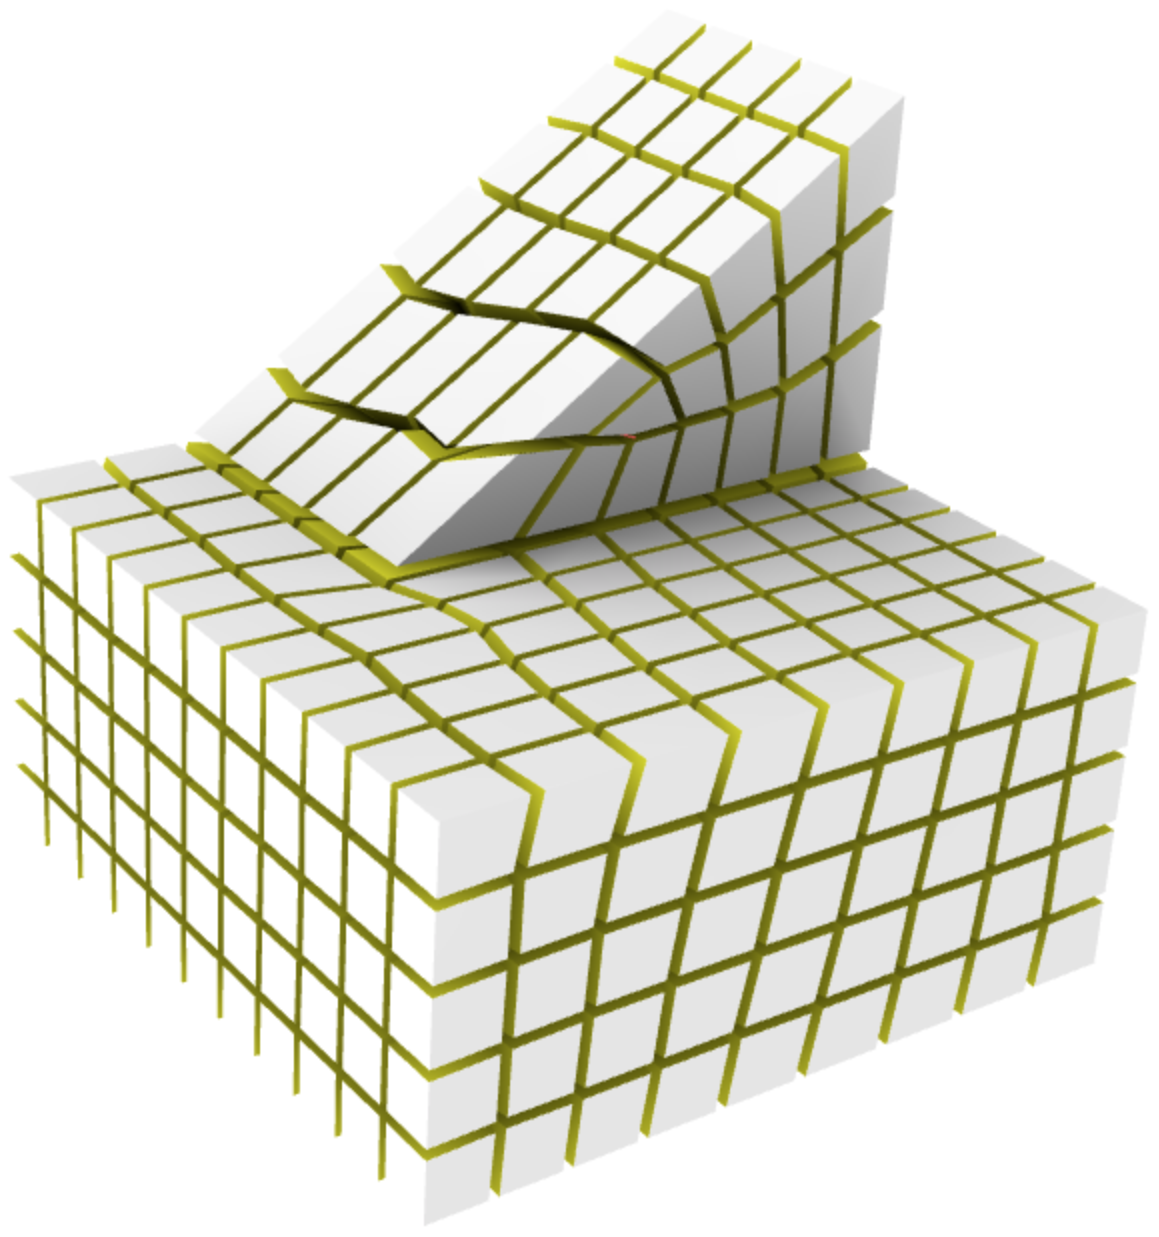
\includegraphics[width=.66\linewidth]{img_spm_ff/slope_northo_front.png}
    %\includegraphics[width=0.8\linewidth]{quads_nonortho_shurik0.PNG}
    %\includegraphics[width=0.8\linewidth]{q_2.PNG}
    \end{minipage}
    %\includegraphics[width=.4\linewidth]{shear_ortho.png}
    %\includegraphics[width=.4\linewidth]{shear_1.png}
    %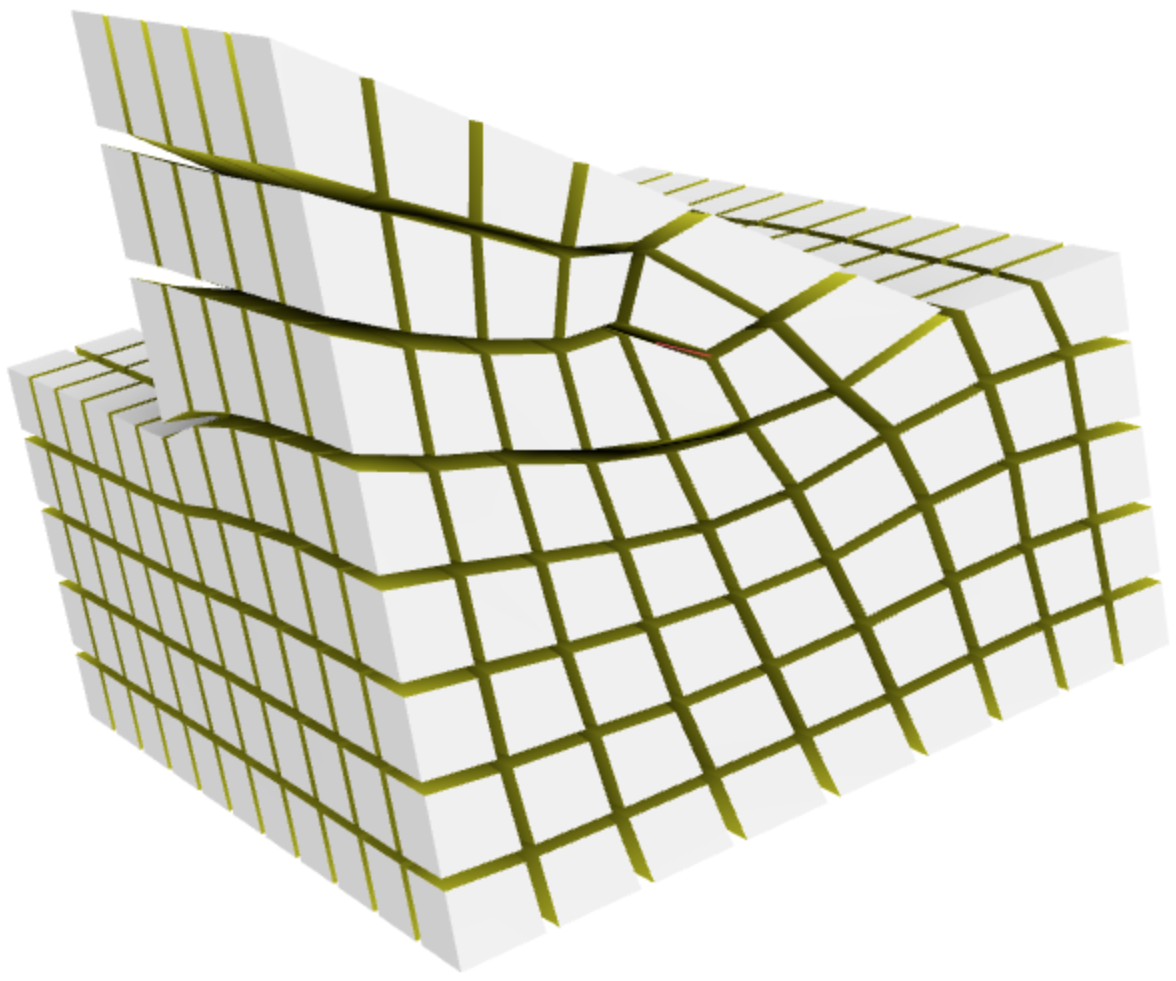
\includegraphics[width=0.4\linewidth]{slope_northo_back.png}
    %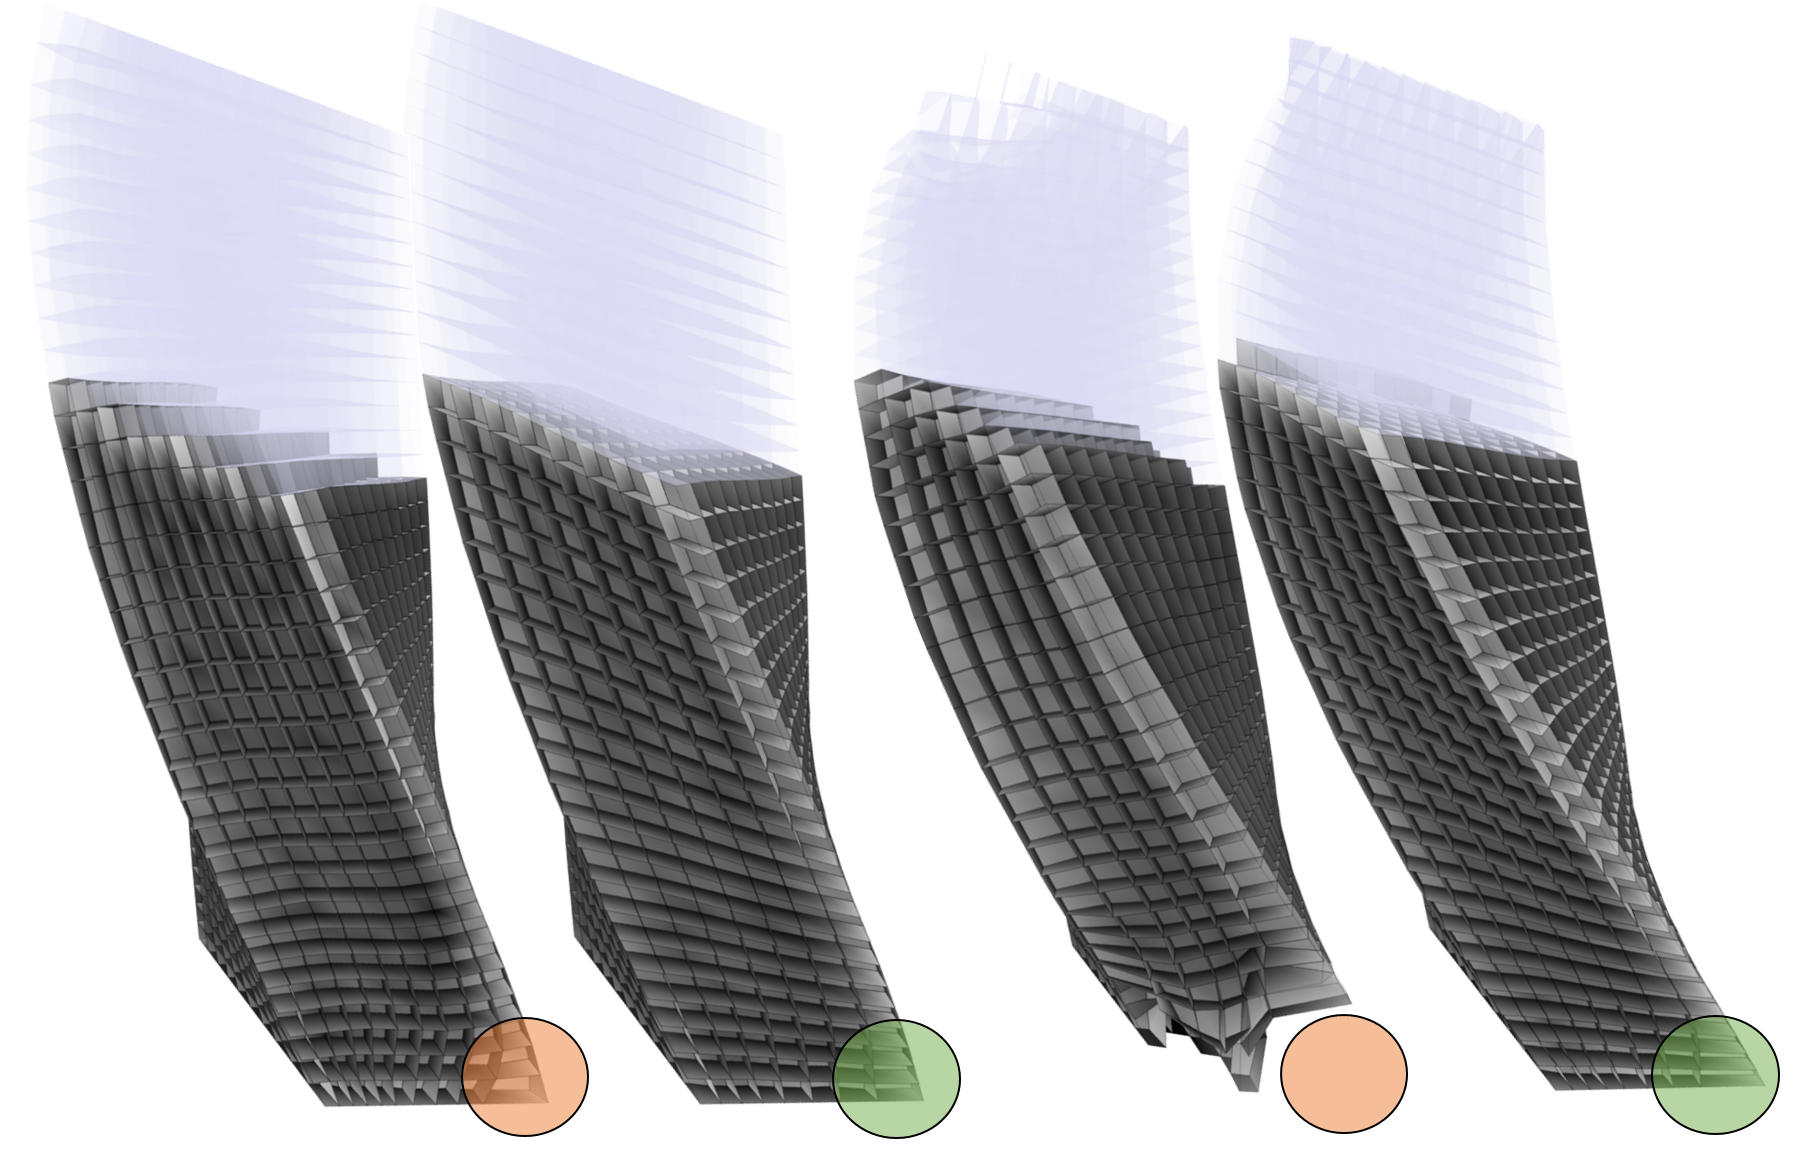
\includegraphics[width=.8\linewidth]{cube_twist_3D.png}
\end{frame} 


\section{Contribution: Quadcover pour des simulations de déformation 2D}
\begin{frame}
    \frametitle{Table des matières}
    \tableofcontents[currentsection, sectionstyle=show/shaded, subsectionstyle=show/show/hide]
\end{frame}
\subsection{Algorithme de quantification 2D rapide, robuste et open source}
\begin{frame}
    \frametitle{Table des matières}
    \tableofcontents[currentsubsection, sectionstyle=show/shaded, subsectionstyle=show/shaded/hide]
\end{frame}
\subsection{Génération de maillage adapté à des déformations avec Quadcover}
\begin{frame}
    \frametitle{Table des matières}
    \tableofcontents[currentsubsection, sectionstyle=show/shaded, subsectionstyle=show/shaded/hide]
\end{frame}

\section{Conclusion}
\begin{frame}
    \frametitle{Table des matières}
    \tableofcontents[currentsection, sectionstyle=show/shaded, subsectionstyle=show/show/hide]
\end{frame}

\end{document}